\documentclass[11pt,a4paper]{article}

% ---------- Essential Packages ----------
\usepackage[margin=0.75in, top=0.75in, bottom=0.75in]{geometry}
\usepackage{graphicx}
\usepackage{booktabs}
\usepackage{tabularx}
\usepackage{array}
\usepackage{float}
\usepackage{enumitem}
\usepackage{xcolor}
\usepackage{amsmath}
\usepackage{amssymb}
\usepackage{tikz}
\usetikzlibrary{shapes.geometric, arrows.meta, positioning, calc, backgrounds, fit, shadows}
\usepackage{hyperref}
\usepackage{fancyhdr}
\usepackage{titlesec}
\usepackage{colortbl}
\usepackage{tcolorbox}
\tcbuselibrary{skins, breakable}
\usepackage{caption}
\usepackage{subcaption}

% ---------- Color Palette (KUET Academic Theme) ----------
\definecolor{kuetblue}{RGB}{20, 52, 100}
\definecolor{kuetnavy}{RGB}{12, 35, 68}
\definecolor{kuetaccent}{RGB}{220, 100, 30}
\definecolor{tableheader}{RGB}{27, 54, 93}
\definecolor{tableheadertext}{RGB}{255, 255, 255}
\definecolor{lightgraybg}{RGB}{248, 249, 250}
\definecolor{bordergray}{RGB}{220, 224, 230}
\definecolor{boxbg}{RGB}{243, 246, 251}

% ---------- Hyperref Setup ----------
\hypersetup{
    colorlinks=true,
    linkcolor=kuetblue,
    citecolor=kuetblue,
    urlcolor=kuetblue
}

% ---------- Header & Footer Styling ----------
\pagestyle{fancy}
\fancyhf{}
\renewcommand{\headrulewidth}{0pt}
\renewcommand{\footrulewidth}{0pt}
\fancyfoot[C]{\thepage}

% ---------- Section Title Formatting ----------
\titleformat{\section}
  {\color{kuetnavy}\normalfont\large\bfseries}{\thesection.}{0.4em}{}[\vspace{-0.35em}\color{kuetblue}\rule{\textwidth}{0.6pt}]

\titleformat{\subsection}
  {\color{kuetblue}\normalfont\normalsize\bfseries}{\thesubsection}{0.35em}{}

\titleformat{\subsubsection}
  {\color{black}\normalfont\small\bfseries}{\thesubsubsection}{0.3em}{}

\titlespacing*{\section}{0pt}{6pt}{3pt}
\titlespacing*{\subsection}{0pt}{4pt}{2pt}
\titlespacing*{\subsubsection}{0pt}{3pt}{1.5pt}

\setlength{\parskip}{2.0pt}
\setlength{\parindent}{0pt}

\graphicspath{{figures/}{ScreenShots/}{./}}

\begin{document}

% ============================================================
% PAGE 1: TITLE PAGE
% ============================================================
\thispagestyle{empty}
{\centering
    \vspace*{0.2cm}
    
    {\Large\textbf{KHULNA UNIVERSITY OF ENGINEERING \& TECHNOLOGY}}\\[0.2cm]
    {\large (KUET)}\\[0.2cm]
    {\large Department of Computer Science and Engineering}\\[0.3cm]
    
    \noindent\makebox[\linewidth]{\color{kuetnavy}\rule{\textwidth}{1.8pt}}\\[0.8cm]
    
    \vspace{0.8cm}
    
    {\fontsize{24pt}{30pt}\selectfont \textbf{\color{kuetnavy}3D Virtual Architectural Walkthrough:}}\\[0.4cm]
    {\fontsize{22pt}{28pt}\selectfont \textbf{\color{kuetblue}Khan Jahan Ali Hall}}\\[1.2cm]
    
    \begin{center}
        \color{kuetaccent}\rule{5cm}{1.2pt}
    \end{center}
    \vspace{0.6cm}
    
    {\large\textbf{Course: CSE 4102}}\\[0.15cm]
    {\normalsize Computer Graphics and Image Processing Laboratory}\\[2.6cm]
    
    \begin{minipage}[t]{0.48\textwidth}
        \raggedright
        \textbf{\large\color{kuetnavy}SUBMITTED BY}\\[0.3cm]
        \textbf{Mehedi Hasan Rabby}\\
        Roll: 2107086\\[0.15cm]
        Year: 4th \quad Term: I\\[0.15cm]
        Department of CSE\\
        Khulna University of Engineering \& Technology
    \end{minipage}
    \hfill
    \begin{minipage}[t]{0.48\textwidth}
        \raggedleft
        \textbf{\large\color{kuetnavy}SUPERVISED BY}\\[0.3cm]
        \textbf{Mr Md. Tajmilur Rahman}\\
        Lecturer, Dept of CSE, KUET\\[0.4cm]
        \textbf{Mr Md. Mubtashim Abrar Nihal}\\
        Lecturer, Dept of CSE, KUET
    \end{minipage}
    
    \vfill
    {\normalsize Khulna -- 9203, Bangladesh}\\[0.15cm]
    {\normalsize October 2026}\par
}

\clearpage

% ============================================================
% PAGE 2: TABLE OF CONTENTS & EXECUTIVE SUMMARY
% ============================================================
\setcounter{tocdepth}{2}
\vspace*{-0.2cm}
{\normalsize
\tableofcontents
}
\vspace{0.6cm}

\begin{tcolorbox}[colback=boxbg, colframe=kuetblue, arc=3pt, title={\textbf{Executive Summary and Project Scope}}, fonttitle=\bfseries]
This report documents the implementation of an interactive 3D virtual walkthrough of \textbf{Khan Jahan Ali Hall} at KUET, created in modern Core Profile OpenGL 3.3, C++, and GLSL. 

In strict adherence to laboratory requirements, the project avoids any external pre-modeled 3D CAD assets (such as OBJ or FBX files). Instead, every object, furniture piece, mechanical fixture, hallway corridor, and campus sports complex is procedurally generated from foundational mathematical formulas using three primary geometric primitives: the \textbf{Unit Cube}, the \textbf{UV Sphere}, and the \textbf{Capped Cylinder}.

The graphics pipeline features per-fragment \textbf{Phong Shading} alongside per-vertex \textbf{Gouraud Shading}, a multi-source lighting system combining directional sunlight with six distance-attenuated point lights, dynamic door kinematics, oscillating fan mechanics, and a first-person collision-bounded navigation system.
\end{tcolorbox}

\vspace{0.4cm}
\begin{tcolorbox}[colback=lightgraybg, colframe=bordergray, arc=3pt]
\textbf{Repository Structure and Core Source Modules:}
\begin{itemize}[leftmargin=1.2em, itemsep=1pt, topsep=1pt]
    \item \texttt{main.cpp}: GLFW window management, keyboard/mouse input dispatch, and render loop.
    \item \texttt{Primitives.cpp / Primitives.h}: Procedural mesh generators for Cube, UV Sphere, and Cylinder.
    \item \texttt{Room.h / Props.h / Fixtures.h}: Scene assembly modules for dorm interior, hallway, and campus quad.
    \item \texttt{default.vert / default.frag}: GLSL 3.3 shaders implementing dual Phong/Gouraud lighting.
\end{itemize}
\end{tcolorbox}




% ============================================================
% PAGE 3: INTRODUCTION & FEATURE MATRIX
% ============================================================
\section{Introduction and Project Scope}

\subsection{Project Motivation and Architectural Context}
The objective of this project is to model and simulate an interactive 3D collegiate residential hall environment---specifically \textbf{Khan Jahan Ali Hall (Room 304)}, along with its enclosed hallway corridor and outdoor quad sports complex---using low-level OpenGL programming. The project demonstrates procedural geometry synthesis, hierarchical coordinate transformations, lighting models, and real-time user interaction.

\subsection{Proposed vs. Implemented Feature Matrix}
Table~\ref{tab:feature_matrix} outlines the proposed milestones compared with the final implementations delivered in the application.

\begin{table}[H]
\centering
\scriptsize
\caption{Comprehensive Comparison of Proposed vs. Implemented Features}
\label{tab:feature_matrix}
\begin{tabularx}{\textwidth}{p{2.5cm}p{3.8cm}p{6.3cm}c}
\toprule
\rowcolor{tableheader}
\textcolor{tableheadertext}{\textbf{Feature Category}} & 
\textcolor{tableheadertext}{\textbf{Proposed Milestone}} & 
\textcolor{tableheadertext}{\textbf{Implemented in Final Project}} & 
\textcolor{tableheadertext}{\textbf{Status}} \\
\midrule
\rowcolor{lightgraybg}
\textbf{3D Primitives} & Procedural generation of basic shapes & Unit Cube (flat normals), UV Sphere (smooth normals), and Capped Cylinder (side radial + cap axial normals) & \textbf{Achieved} \\
\textbf{Room 304 Interior} & 4 beds, study tables, chairs, boundaries & 4 wooden beds with recessed mattresses \& under-bed luggage, 4 workstations with PCs \& CPUs, 2 almirahs, 2 tea tables & \textbf{Exceeded} \\
\rowcolor{lightgraybg}
\textbf{Corridor Hallway} & Wall opening exit representation & Fully enclosed corridor with terrazzo runner, opposite dorm doors (303, 305), notice board, fire extinguisher, water dispenser & \textbf{Exceeded} \\
\textbf{Balcony \& Quad} & Balcony terrace with railing & Cantilever corbels, patio mosaic, planters, full quad athletic field (running track, soccer pitch, cricket pitch \& wickets, floodlights, hall wings) & \textbf{Exceeded} \\
\rowcolor{lightgraybg}
\textbf{Dynamic Animations} & Static scene or single rotation & Smooth exponential-decay door opening for both Balcony and Main Door, 4 continuous ceiling fans, and dual-motion oscillating table fan & \textbf{Exceeded} \\
\textbf{Illumination Models} & Single directional light & Directional Sunlight + 6 attenuated Point Lights (4 room tubes, 1 corridor light, 1 balcony sconce). Independent 4-gang electrical switchboard toggles & \textbf{Exceeded} \\
\rowcolor{lightgraybg}
\textbf{Shading Techniques} & Basic lighting implementation & Runtime-switchable per-pixel Phong Shading ($P$ key) and per-vertex Gouraud Shading ($G$ key) with normal matrix corrections & \textbf{Achieved} \\
\textbf{Emissive Materials} & Not initially planned & Selective emissive rendering bypassing shading for active tube light bulbs, PC screens, router status LEDs, switchboard indicators, and sun & \textbf{Achieved} \\
\rowcolor{lightgraybg}
\textbf{Interactive Camera} & Simple keyboard camera navigation & First-person walk/strafe with pitch/yaw clamping, level horizontal motion vector, and multi-zone portal collision logic across doors & \textbf{Achieved} \\
\bottomrule
\end{tabularx}
\end{table}




% ============================================================
% PAGE 4: PRIMITIVE 1 - THE UNIT CUBE
% ============================================================
\section{Mathematical Computation of 3D Geometric Primitives}

Every 3D object in this virtual environment is procedurally constructed from three primitive meshes implemented in \texttt{Primitives.cpp}: the \textbf{Cube}, the \textbf{Sphere}, and the \textbf{Cylinder}.

\subsection{Primitive 1: The Unit Cube (Axis-Aligned Box)}

\subsubsection{Vertex Coordinates and Face Normal Vectors}
The unit cube occupies local coordinates $X \in [-0.5, 0.5]$, $Y \in [-0.5, 0.5]$, and $Z \in [-0.5, 0.5]$. Because a box has sharp $90^\circ$ edges, vertices cannot share surface normals across adjoining faces without producing blurred lighting artifacts. Consequently, each of the 6 faces requires 4 dedicated vertices with identical outward-pointing normal vectors:
\begin{align}
    \mathbf{n}_{\text{front}}  &= (0.0, 0.0, +1.0) & \mathbf{n}_{\text{back}}   &= (0.0, 0.0, -1.0) \\
    \mathbf{n}_{\text{top}}    &= (0.0, +1.0, 0.0) & \mathbf{n}_{\text{bottom}} &= (0.0, -1.0, 0.0) \\
    \mathbf{n}_{\text{right}}  &= (+1.0, 0.0, 0.0) & \mathbf{n}_{\text{left}}   &= (-1.0, 0.0, 0.0)
\end{align}
This yields a total of $6 \times 4 = 24$ vertices. For each planar face, the 4 vertices form a counter-clockwise (CCW) quad decomposed into two triangles: $\triangle(v_0, v_1, v_2)$ and $\triangle(v_2, v_3, v_0)$.

\begin{table}[H]
\centering
\scriptsize
\caption{Unit Cube Vertex and Triangle Index Specification (VBO and EBO Layout)}
\label{tab:cube_vertices}
\begin{tabular}{lccccc}
\toprule
\rowcolor{tableheader}
\textcolor{tableheadertext}{\textbf{Face}} & 
\textcolor{tableheadertext}{\textbf{Vertex IDs}} & 
\textcolor{tableheadertext}{\textbf{Local Position $(x,y,z)$}} & 
\textcolor{tableheadertext}{\textbf{Surface Normal $\mathbf{n}$}} & 
\textcolor{tableheadertext}{\textbf{Triangle Decomposition}} & 
\textcolor{tableheadertext}{\textbf{EBO Indices}} \\
\midrule
\rowcolor{lightgraybg}
Front ($+Z$) & $0, 1, 2, 3$ & $(\pm 0.5, \pm 0.5, +0.5)$ & $(0.0, 0.0, +1.0)$ & $\triangle(0,1,2), \triangle(2,3,0)$ & $0,1,2, 2,3,0$ \\
Back ($-Z$)  & $4, 5, 6, 7$ & $(\pm 0.5, \pm 0.5, -0.5)$ & $(0.0, 0.0, -1.0)$ & $\triangle(4,5,6), \triangle(6,7,4)$ & $4,5,6, 6,7,4$ \\
\rowcolor{lightgraybg}
Top ($+Y$)   & $8, 9, 10, 11$ & $(\pm 0.5, +0.5, \pm 0.5)$ & $(0.0, +1.0, 0.0)$ & $\triangle(8,9,10), \triangle(10,11,8)$ & $8,9,10, 10,11,8$ \\
Bottom ($-Y$)& $12, 13, 14, 15$ & $(\pm 0.5, -0.5, \pm 0.5)$ & $(0.0, -1.0, 0.0)$ & $\triangle(12,13,14), \triangle(14,15,12)$ & $12,13,14, 14,15,12$ \\
\rowcolor{lightgraybg}
Right ($+X$) & $16, 17, 18, 19$ & $(+0.5, \pm 0.5, \pm 0.5)$ & $(+1.0, 0.0, 0.0)$ & $\triangle(16,17,18), \triangle(18,19,16)$ & $16,17,18, 18,19,16$ \\
Left ($-X$)  & $20, 21, 22, 23$ & $(-0.5, \pm 0.5, \pm 0.5)$ & $(-1.0, 0.0, 0.0)$ & $\triangle(20,21,22), \triangle(22,23,20)$ & $20,21,22, 22,23,20$ \\
\bottomrule
\end{tabular}
\end{table}

\begin{figure}[H]
\centering
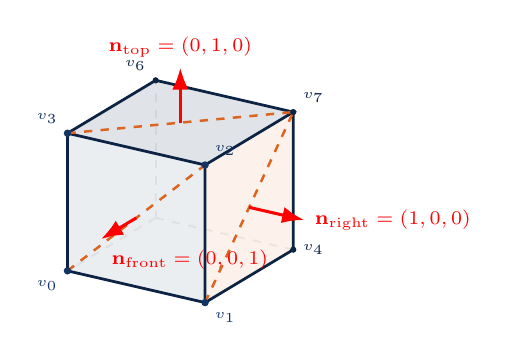
\begin{tikzpicture}[x={(0.78cm,-0.18cm)}, y={(0cm,0.78cm)}, z={(-0.50cm,-0.30cm)}, scale=1.12, >=Latex]
    \coordinate (V0) at (-1, -1, 1);
    \coordinate (V1) at ( 1, -1, 1);
    \coordinate (V2) at ( 1,  1, 1);
    \coordinate (V3) at (-1,  1, 1);
    \coordinate (V4) at ( 1, -1, -1);
    \coordinate (V5) at (-1, -1, -1);
    \coordinate (V6) at (-1,  1, -1);
    \coordinate (V7) at ( 1,  1, -1);

    % Back edges
    \draw[dashed, color=gray!70, line width=0.7pt] (V5) -- (V4);
    \draw[dashed, color=gray!70, line width=0.7pt] (V5) -- (V6);
    \draw[dashed, color=gray!70, line width=0.7pt] (V5) -- (V0);

    % Shaded faces
    \fill[kuetblue!10, opacity=0.85] (V0) -- (V1) -- (V2) -- (V3) -- cycle;
    \fill[kuetnavy!15, opacity=0.85] (V3) -- (V2) -- (V7) -- (V6) -- cycle;
    \fill[kuetaccent!10, opacity=0.85] (V1) -- (V4) -- (V7) -- (V2) -- cycle;

    % Visible edges
    \draw[thick, color=kuetnavy, line width=1.0pt] (V0) -- (V1) -- (V2) -- (V3) -- cycle;
    \draw[thick, color=kuetnavy, line width=1.0pt] (V3) -- (V6) -- (V7) -- (V2);
    \draw[thick, color=kuetnavy, line width=1.0pt] (V1) -- (V4) -- (V7);

    % Triangulation diagonal dashes
    \draw[dashed, color=kuetaccent, line width=0.9pt] (V0) -- (V2);
    \draw[dashed, color=kuetaccent, line width=0.9pt] (V3) -- (V7);
    \draw[dashed, color=kuetaccent, line width=0.9pt] (V1) -- (V7);

    % Normal vectors
    \draw[->, line width=1.1pt, color=red] (0, 0, 1) -- (0, 0, 1.8) node[below right, font=\scriptsize] {$\mathbf{n}_{\text{front}} = (0, 0, 1)$};
    \draw[->, line width=1.1pt, color=red] (0, 1, 0) -- (0, 1.8, 0) node[above, font=\scriptsize] {$\mathbf{n}_{\text{top}} = (0, 1, 0)$};
    \draw[->, line width=1.1pt, color=red] (1, 0, 0) -- (1.8, 0, 0) node[right, font=\scriptsize] {$\mathbf{n}_{\text{right}} = (1, 0, 0)$};

    % Vertex markers and labels
    \fill[kuetblue] (V0) circle (1.2pt) node[below left, font=\tiny] {$v_0$};
    \fill[kuetblue] (V1) circle (1.2pt) node[below right, font=\tiny] {$v_1$};
    \fill[kuetblue] (V2) circle (1.2pt) node[above right, font=\tiny] {$v_2$};
    \fill[kuetblue] (V3) circle (1.2pt) node[above left, font=\tiny] {$v_3$};
    \fill[kuetnavy] (V4) circle (1.0pt) node[right, font=\tiny] {$v_4$};
    \fill[kuetnavy] (V6) circle (1.0pt) node[above left, font=\tiny] {$v_6$};
    \fill[kuetnavy] (V7) circle (1.0pt) node[above right, font=\tiny] {$v_7$};
\end{tikzpicture}
\caption{Unit Cube geometry with CCW triangle tessellation ($\triangle(0,1,2)$, $\triangle(2,3,0)$) and orthogonal face normals.}
\label{fig:cube_math}
\end{figure}

\subsubsection{EBO Indexing and Buffer Memory Optimization}
Without an index buffer, rendering 12 triangles requires $12 \times 3 = 36$ vertices. Each vertex contains 6 32-bit floats (3 position + 3 normal), totaling $36 \times 6 \times 4 = 864$ bytes. With an Element Buffer Object (EBO):
\begin{equation}
    \text{VBO} = 24 \times 6 \times 4 = 576\text{ B}, \quad \text{EBO} = 36 \times 4 = 144\text{ B} \implies \text{Total} = 720\text{ B (16.7\% reduction)}
\end{equation}




% ============================================================
% PAGE 5: PRIMITIVE 2 - THE UV SPHERE
% ============================================================
\subsection{Primitive 2: The UV Sphere (Latitude-Longitude Mesh)}

\subsubsection{Continuous Parametric Equations and Analytical Normal Derivation}
The UV Sphere of radius $r = 1.0$ centered at the origin is parameterized by polar angle (colatitude) $\theta \in [0, \pi]$ and azimuthal angle (longitude) $\phi \in [0, 2\pi]$:
\begin{equation}
    \mathbf{p}(\theta, \phi) = \begin{pmatrix} x(\theta, \phi) \\ y(\theta, \phi) \\ z(\theta, \phi) \end{pmatrix} = \begin{pmatrix} r \sin\theta \cos\phi \\ r \cos\theta \\ r \sin\theta \sin\phi \end{pmatrix}
\end{equation}
The implicit surface representation is $F(x, y, z) = x^2 + y^2 + z^2 - r^2 = 0$. The analytical outward unit normal vector $\mathbf{n}$ is obtained by normalizing the gradient $\nabla F$:
\begin{equation}
    \nabla F = \begin{pmatrix} \frac{\partial F}{\partial x} \\ \frac{\partial F}{\partial y} \\ \frac{\partial F}{\partial z} \end{pmatrix} = \begin{pmatrix} 2x \\ 2y \\ 2z \end{pmatrix} \implies \mathbf{n} = \frac{\nabla F}{\|\nabla F\|} = \frac{(2x, 2y, 2z)}{\sqrt{4x^2 + 4y^2 + 4z^2}} = \frac{(x, y, z)}{r} = \begin{pmatrix} \sin\theta \cos\phi \\ \cos\theta \\ \sin\theta \sin\phi \end{pmatrix}
\end{equation}
Thus, for any point on a unit sphere ($r=1.0$), the outward normal vector is numerically identical to its position vector: $\mathbf{n} = \mathbf{p}$.

\subsubsection{Discrete Tessellation Algorithm and Coordinate Calculations}
The continuous sphere is tessellated into $N_{\text{stacks}} = 14$ latitude rings and $N_{\text{sectors}} = 18$ longitude segments. For discrete indices $i \in [0, N_{\text{stacks}}]$ and $j \in [0, N_{\text{sectors}}]$:
\begin{equation}
    \theta_i = \frac{i \cdot \pi}{N_{\text{stacks}}}, \quad \phi_j = \frac{j \cdot 2\pi}{N_{\text{sectors}}}
\end{equation}

\begin{figure}[H]
\centering
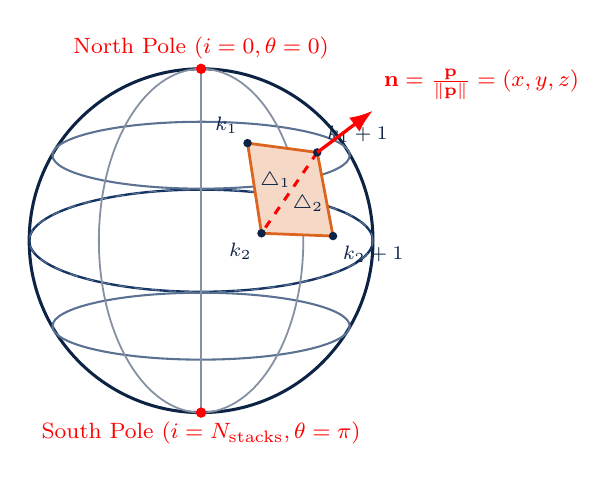
\begin{tikzpicture}[scale=1.18, >=Latex]
    \draw[line width=1.1pt, color=kuetnavy] (0,0) circle (1.85cm);
    
    \draw[color=kuetblue, line width=0.85pt] (0,0) ellipse (1.85cm and 0.55cm);
    \draw[color=kuetblue!70, dashed] (0,0) ellipse (1.85cm and 0.55cm);
    \draw[color=kuetblue!70, line width=0.75pt] (0,0.92) ellipse (1.60cm and 0.36cm);
    \draw[color=kuetblue!70, line width=0.75pt] (0,-0.92) ellipse (1.60cm and 0.36cm);
    
    \draw[color=kuetnavy!50, line width=0.65pt] (0,1.85) arc (90:-90:1.1cm and 1.85cm);
    \draw[color=kuetnavy!50, line width=0.65pt] (0,1.85) arc (90:-90:0.0cm and 1.85cm);
    \draw[color=kuetnavy!50, line width=0.65pt] (0,1.85) arc (90:270:1.1cm and 1.85cm);

    \fill[red] (0,1.85) circle (1.6pt) node[above, font=\footnotesize] {North Pole ($i=0, \theta=0$)};
    \fill[red] (0,-1.85) circle (1.6pt) node[below, font=\footnotesize] {South Pole ($i=N_{\text{stacks}}, \theta=\pi$)};

    \coordinate (K1) at (0.50, 1.05);
    \coordinate (K2) at (0.65, 0.08);
    \coordinate (K1P) at (1.25, 0.95);
    \coordinate (K2P) at (1.42, 0.05);

    \fill[kuetaccent!25, draw=kuetaccent, line width=1.0pt] (K1) -- (K2) -- (K2P) -- (K1P) -- cycle;
    \draw[line width=1.1pt, dashed, color=red] (K1P) -- (K2);

    \fill[kuetnavy] (K1) circle (1.3pt) node[above left, font=\scriptsize] {$k_1$};
    \fill[kuetnavy] (K2) circle (1.3pt) node[below left, font=\scriptsize] {$k_2$};
    \fill[kuetnavy] (K1P) circle (1.3pt) node[above right, font=\scriptsize] {$k_1+1$};
    \fill[kuetnavy] (K2P) circle (1.3pt) node[below right, font=\scriptsize] {$k_2+1$};

    \node[font=\scriptsize, color=kuetnavy] at (0.80, 0.65) {$\triangle_1$};
    \node[font=\scriptsize, color=kuetnavy] at (1.15, 0.40) {$\triangle_2$};

    \draw[->, line width=1.2pt, color=red] (K1P) -- ++(0.60, 0.45) node[above right, font=\footnotesize] {$\mathbf{n} = \frac{\mathbf{p}}{\|\mathbf{p}\|} = (x, y, z)$};
\end{tikzpicture}
\caption{UV Sphere grid discretization into latitude stacks and longitude sectors, showing individual quad split into two CCW triangles: $\triangle_1(k_1, k_2, k_1+1)$ and $\triangle_2(k_1+1, k_2, k_2+1)$.}
\label{fig:sphere_math}
\end{figure}

\subsubsection{Quad Index Topology and Polar Singularities}
Each quadrilateral patch between adjacent stacks $i, i+1$ and sectors $j, j+1$ is indexed via $k_1 = i(N_{\text{sectors}} + 1) + j$ and $k_2 = k_1 + N_{\text{sectors}} + 1$. The quad is split into two CCW triangles: $\triangle_1(k_1, k_2, k_1+1)$ and $\triangle_2(k_1+1, k_2, k_2+1)$. At the North Pole ($i = 0$), $\triangle_1$ is omitted; at the South Pole ($i = N_{\text{stacks}}-1$), $\triangle_2$ is omitted:
\begin{equation}
    \text{Vertices} = (14 + 1)(18 + 1) = \mathbf{285}, \quad \text{Triangles} = 2 \cdot 18 \cdot (14 - 1) = \mathbf{468} \implies \mathbf{1404 \text{ EBO indices}}
\end{equation}




% ============================================================
% PAGE 6: PRIMITIVE 3 - THE CAPPED CYLINDER
% ============================================================
\subsection{Primitive 3: The Capped Cylinder}

\subsubsection{Side Surface Equations and Outward Radial Normals}
A cylinder of radius $r = 1.0$ and height $h = 1.0$ aligned along the $Y$-axis has side surface parametric equations:
\begin{equation}
    x(\theta_j) = r \cos\theta_j, \quad z(\theta_j) = r \sin\theta_j, \quad y \in [-h/2, +h/2], \quad \theta_j = \frac{j \cdot 2\pi}{N_{\text{sectors}}}
\end{equation}
The side wall outward normal points purely radially across the $XZ$ plane, with no vertical component:
\begin{equation}
    \mathbf{n}_{\text{side}}(\theta_j) = \left(\frac{x}{\sqrt{x^2+z^2}}, 0.0, \frac{z}{\sqrt{x^2+z^2}}\right) = \left(\cos\theta_j, 0.0, \sin\theta_j\right)
\end{equation}

\subsubsection{Top and Bottom End Cap Planar Fans}
To avoid blurred edge shading, the flat end caps are generated using distinct vertices with axial normals:
\begin{align}
    \text{Top Cap ($y = +h/2$):}    \quad \mathbf{n}_{\text{top}} &= (0.0, +1.0, 0.0), \quad C_{\text{top}} = (0.0, +0.5, 0.0) \\
    \text{Bottom Cap ($y = -h/2$):} \quad \mathbf{n}_{\text{bot}} &= (0.0, -1.0, 0.0), \quad C_{\text{bot}} = (0.0, -0.5, 0.0)
\end{align}

\begin{figure}[H]
\centering
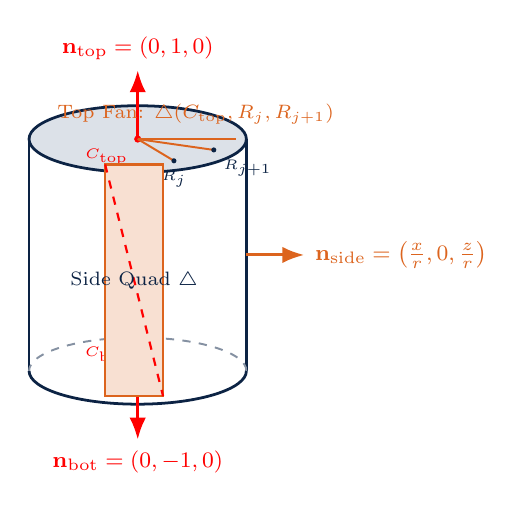
\begin{tikzpicture}[scale=0.92, >=Latex]
    \coordinate (TopCenter) at (0, 1.6);
    \coordinate (BotCenter) at (0, -1.6);

    \draw[line width=1.0pt, color=kuetnavy] (-1.5, 1.6) -- (-1.5, -1.6);
    \draw[line width=1.0pt, color=kuetnavy] (1.5, 1.6) -- (1.5, -1.6);

    \draw[color=kuetnavy, line width=1.0pt] (1.5, -1.6) arc (0:-180:1.5cm and 0.46cm);
    \draw[color=kuetnavy!50, dashed, line width=0.7pt] (1.5, -1.6) arc (0:180:1.5cm and 0.46cm);

    \fill[kuetblue!15, draw=kuetnavy, line width=1.0pt] (0, 1.6) ellipse (1.5cm and 0.46cm);

    \fill[red] (TopCenter) circle (1.4pt) node[below left, font=\tiny] {$C_{\text{top}}$};
    \draw[->, line width=1.1pt, color=red] (TopCenter) -- ++(0, 0.95) node[above, font=\footnotesize] {$\mathbf{n}_{\text{top}} = (0, 1, 0)$};

    \fill[red] (BotCenter) circle (1.4pt) node[above left, font=\tiny] {$C_{\text{bot}}$};
    \draw[->, line width=1.1pt, color=red] (BotCenter) -- ++(0, -0.95) node[below, font=\footnotesize] {$\mathbf{n}_{\text{bot}} = (0, -1, 0)$};

    \coordinate (R1) at (0.50, 1.30);
    \coordinate (R2) at (1.05, 1.45);
    \coordinate (R3) at (1.35, 1.60);
    \draw[color=kuetaccent, line width=0.7pt] (TopCenter) -- (R1);
    \draw[color=kuetaccent, line width=0.7pt] (TopCenter) -- (R2);
    \draw[color=kuetaccent, line width=0.7pt] (TopCenter) -- (R3);
    \fill[kuetnavy] (R1) circle (1.0pt) node[below, font=\tiny] {$R_j$};
    \fill[kuetnavy] (R2) circle (1.0pt) node[below right, font=\tiny] {$R_{j+1}$};
    \node[font=\scriptsize, color=kuetaccent] at (0.8, 1.95) {Top Fan: $\triangle(C_{\text{top}}, R_j, R_{j+1})$};

    \coordinate (SW_T1) at (-0.45, 1.25);
    \coordinate (SW_T2) at (0.35, 1.25);
    \coordinate (SW_B1) at (-0.45, -1.95);
    \coordinate (SW_B2) at (0.35, -1.95);

    \fill[kuetaccent!20, draw=kuetaccent, line width=0.8pt] (SW_T1) -- (SW_T2) -- (SW_B2) -- (SW_B1) -- cycle;
    \draw[dashed, line width=0.8pt, color=red] (SW_T1) -- (SW_B2);
    \node[font=\scriptsize, color=kuetnavy] at (-0.05, -0.35) {Side Quad $\triangle$};

    \coordinate (SideFrag) at (1.5, 0.0);
    \draw[->, line width=1.1pt, color=kuetaccent] (SideFrag) -- ++(0.8, 0.0) node[right, font=\footnotesize] {$\mathbf{n}_{\text{side}} = \left(\frac{x}{r}, 0, \frac{z}{r}\right)$};
\end{tikzpicture}
\caption{Capped Cylinder mesh showing outward radial normals on side walls, axial normals on end caps, and CCW triangle fan and strip decomposition.}
\label{fig:cylinder_math}
\end{figure}

\subsubsection{Triangle Winding Order and Index Formulas}
For $N_{\text{sectors}} = 18$:
\begin{enumerate}[leftmargin=1.2em, itemsep=0.5pt, topsep=0.5pt]
    \item \textbf{Side Wall Triangles:} Each sector connects $\text{top}_1 = 2j, \text{bot}_1 = 2j+1, \text{top}_2 = 2(j+1), \text{bot}_2 = 2(j+1)+1$ into two CCW triangles: $\triangle(\text{top}_1, \text{bot}_1, \text{top}_2)$ and $\triangle(\text{top}_2, \text{bot}_1, \text{bot}_2)$, yielding $18 \times 2 = 36$ triangles ($108$ indices).
    \item \textbf{Top Cap Fan:} Connects $C_{\text{top}}$ with rim vertices $R_j$ and $R_{j+1}$: $\triangle(C_{\text{top}}, R_j, R_{j+1})$, yielding 18 triangles ($54$ indices).
    \item \textbf{Bottom Cap Fan:} Winding order reversed for counter-clockwise visibility: $\triangle(C_{\text{bot}}, R_{j+1}, R_j)$, yielding 18 triangles ($54$ indices).
\end{enumerate}
\begin{equation}
    \text{Total Vertices} = 2(19) + 1 + 19 + 1 + 19 = \mathbf{78 \text{ vertices}}, \quad \text{Total EBO Indices} = 108 + 54 + 54 = \mathbf{216 \text{ indices}}
\end{equation}




% ============================================================
% PAGE 7: PRIMITIVES SUMMARY & TRANSFORMATION PIPELINE
% ============================================================
\subsection{Primitive Geometry and Buffer Memory Footprint Analysis}
Table~\ref{tab:primitives_summary} summarizes geometric specifications, vertex counts, index buffers, and GPU memory footprints across the three procedural primitive meshes.

\begin{table}[H]
\centering
\scriptsize
\caption{Consolidated Summary of Procedural Primitive Mesh Specifications}
\label{tab:primitives_summary}
\begin{tabularx}{\textwidth}{lcccccX}
\toprule
\rowcolor{tableheader}
\textcolor{tableheadertext}{\textbf{Primitive}} & 
\textcolor{tableheadertext}{\textbf{Resolution}} & 
\textcolor{tableheadertext}{\textbf{Vertices}} & 
\textcolor{tableheadertext}{\textbf{Triangles}} & 
\textcolor{tableheadertext}{\textbf{EBO Indices}} & 
\textcolor{tableheadertext}{\textbf{VBO+EBO (Bytes)}} & 
\textcolor{tableheadertext}{\textbf{Primary Use Cases in Scene}} \\
\midrule
\rowcolor{lightgraybg}
\textbf{Unit Cube} & 6 flat faces & 24 & 12 & 36 & 720 & Walls, doors, floors, table tops, beds, shelves, books, suitcase bodies, CPU chassis, notice board, goals \\
\textbf{UV Sphere} & $14 \times 18$ grid & 285 & 468 & 1404 & 12,456 & Ceiling fan motor hubs, potted plant foliage, outdoor trees, light bulbs, door knobs, pushpins, sun \\
\rowcolor{lightgraybg}
\textbf{Cylinder}  & 18 sectors & 78 & 72 & 216 & 2,736 & Bed posts, chair/table legs, fan drop rods, water bottles, fire extinguisher, cricket wickets, floodlight masts \\
\midrule
\textbf{Total Static Cache} & --- & \textbf{387} & \textbf{552} & \textbf{1656} & \textbf{15,912} & \textbf{Entire 3D world rendered from 15.5 KB primitive cache} \\
\bottomrule
\end{tabularx}
\end{table}

\begin{tcolorbox}[colback=boxbg, colframe=kuetblue, arc=3pt, title={\textbf{Engineering Principle: Zero External CAD Asset Dependency}}, fonttitle=\bfseries]
By maintaining static Vertex Array Objects (VAOs) for these three primitives uploaded to GPU VRAM once during initialization, the entire 3D virtual world requires zero external 3D model files (OBJ, FBX) or textures. This eliminates disk I/O overhead and delivers stable 60.0 FPS rendering performance.
\end{tcolorbox}

\subsection{Coordinate Transformation Pipeline}
Every object in the virtual world is positioned and shaped using standard 3D affine matrix transformations. A vertex in local primitive space $\mathbf{v}_{\text{local}}$ is transformed to normalized device coordinates $\mathbf{v}_{\text{clip}}$ via the Model-View-Projection pipeline:
\begin{equation}
    \mathbf{v}_{\text{clip}} = \mathbf{P} \cdot \mathbf{V} \cdot \mathbf{M} \cdot \begin{pmatrix} \mathbf{v}_{\text{local}} \\ 1 \end{pmatrix}
\end{equation}
where:
\begin{enumerate}[leftmargin=1.2em, itemsep=1.0pt, topsep=1.0pt]
    \item \textbf{Model Matrix $\mathbf{M} = \mathbf{T}(t_x, t_y, t_z) \cdot \mathbf{R}_y(\theta) \cdot \mathbf{S}(s_x, s_y, s_z)$}: Scales the unit primitive to desired physical dimensions, rotates it to target orientation, and translates it to world coordinates.
    \item \textbf{View Matrix $\mathbf{V}$}: Generated using camera look-at transformation:
    $\mathbf{V} = \begin{pmatrix} \mathbf{R}_x & \mathbf{R}_y & \mathbf{R}_z & -\mathbf{R} \cdot \mathbf{P}_{\text{cam}} \\ 0 & 0 & 0 & 1 \end{pmatrix}$.
    \item \textbf{Projection Matrix $\mathbf{P}$}: Perspective projection ($\text{FOV} = 45^\circ$, near plane $z_{\text{near}} = 0.1$, far plane $z_{\text{far}} = 300.0$):
    \begin{equation}
        \mathbf{P} = \begin{pmatrix} 
        \frac{1}{\text{aspect} \cdot \tan(\text{FOV}/2)} & 0 & 0 & 0 \\
        0 & \frac{1}{\tan(\text{FOV}/2)} & 0 & 0 \\
        0 & 0 & -\frac{z_{\text{far}} + z_{\text{near}}}{z_{\text{far}} - z_{\text{near}}} & -\frac{2 z_{\text{far}} z_{\text{near}}}{z_{\text{far}} - z_{\text{near}}} \\
        0 & 0 & -1 & 0
        \end{pmatrix}
    \end{equation}
\end{enumerate}




% ============================================================
% PAGE 8: HIERARCHICAL MODELING & SCENE CONSTRUCTION
% ============================================================
\section{Hierarchical Modeling and Architectural Scene Construction}

\subsection{Interior Environment: Khan Jahan Ali Hall (Room 304)}
Room 304 represents a collegiate quadruple room with dimensions $16.0 \times 6.0 \times 18.0$ units ($X \in [-8.0, 8.0]$, $Y \in [-2.5, 3.5]$, $Z \in [-9.0, 9.0]$). All interior assets are constructed hierarchically using primitives.

\subsubsection{Student Bed Assemblies with Recessed Mattresses and Under-Bed Luggage}
Four identical student beds are placed symmetrically across the room at centers $(-5.5, -1.8, -5.0)$, $(-5.5, -1.8, 2.0)$, $(5.5, -1.8, -5.0)$, and $(5.5, -1.8, 2.0)$:
\begin{itemize}[leftmargin=1.2em, itemsep=0.5pt, topsep=0.5pt]
    \item \textbf{Posts and Frame Rails:} 4 vertical cylindrical legs ($h = 1.2, r = 0.08$) and rectangular timber side runners.
    \item \textbf{Headboard and Footboard:} Scaled cubes with beveled crown moldings.
    \item \textbf{Recessed Mattress and Pillows:} A scaled mattress cube ($1.8 \times 0.28 \times 3.6$) recessed within side rails, draped with dark blue bedding and a soft white rounded pillow.
    \item \textbf{Under-Bed Hard-Shell Trolley Luggage:} Positioned beneath each bed. Each luggage features distinct colors (Navy, Maroon, Charcoal, Teal), a grooved shell, corner bumpers, rubber wheels, and a telescoping handle.
\end{itemize}

\subsubsection{Workstations: Study Desks, Desktop PCs, and Chairs}
Four complete computing workstations are aligned adjacent to the student beds:
\begin{itemize}[leftmargin=1.2em, itemsep=0.5pt, topsep=0.5pt]
    \item \textbf{Study Desks:} Timber tables with polished tops at $y = -1.225$, dual side leg panels, and privacy backboards.
    \item \textbf{Desktop PCs:} Monitor with slim bezel, neck, baseplate, and an \textbf{emissive glowing blue display screen} ($0.0, 0.72, 1.0$), accompanied by a black ATX mid-tower CPU case, optical drive slot, keyboard tray, and mouse.
    \item \textbf{Ergonomic Chairs:} Contoured seat cushion ($y = -1.70$), backrest slats, and cylindrical support legs.
\end{itemize}

\subsubsection{Mechanical and Electrical Fixtures}
\begin{itemize}[leftmargin=1.2em, itemsep=0.5pt, topsep=0.5pt]
    \item \textbf{Ceiling and Table Fans:} 4 ceiling fans suspended from drop rods, rotating continuously. A detailed table fan on the central study table executes dual kinetic motion (high-speed blade rotation and sinusoidal horizontal case oscillation).
    \item \textbf{4-Gang Electrical Switchboard:} Mounted at eye level $(4.0, 0.0, -8.82)$. Contains 4 toggle switches controlling the tube lights independently, with live LED indicators (green when active, red when off).
    \item \textbf{Wall-Mounted Wi-Fi Router:} Sleek chassis on a wall bracket with 4 angled antennas and illuminated status indicator lights.
\end{itemize}

\subsection{Hallway Corridor Environment}
\begin{itemize}[leftmargin=1.2em, itemsep=0.5pt, topsep=0.5pt]
    \item \textbf{Architectural Layout:} Spans $X \in [-12.0, 12.0]$, $Z \in [-14.5, -9.0]$, connecting Room 304 with adjacent rooms (302, 306) and opposite rooms (303, 305).
    \item \textbf{Anti-Z-Fighting Terrazzo Runner:} A central floor runner strip ($24.0 \times 2.0$ units) is positioned at $y = -2.48$, precisely $\Delta y = 0.02$ units above the base floor slab, eliminating coplanar depth-buffer fighting.
    \item \textbf{Corridor Assets:} Wall-mounted notice board with pinned announcements, pressure-gauge fire extinguisher, and drinking water dispenser with blue water carboy.
\end{itemize}

\subsection{Balcony Terrace and Quad Athletic Sports Complex}
Beyond the sliding glass balcony door at $z = +9.0$, Room 304 extends into an outdoor balcony terrace ($5.2 \times 4.6$ units) overlooking the university courtyard below at $y = -5.85$. The outdoor sports complex features:
\begin{itemize}[leftmargin=1.2em, itemsep=0.5pt, topsep=0.5pt]
    \item \textbf{Athletic Field:} A 400m running track with green infield soccer pitch and regulation goal posts.
    \item \textbf{Cricket Strip:} Central clay pitch with regulation timber wickets and bails.
    \item \textbf{Surrounding Architecture:} Multi-story residential hall wings (South Wing 5 floors, East and West Wings 2 floors, North Wing with clock tower and archway), four 30m corner floodlight masts, outdoor trees, and sky dome.
\end{itemize}




% ============================================================
% PAGE 9: ILLUMINATION & SHADING MODELS (PART 1)
% ============================================================
\section{Illumination and Shading Models: Mathematical Formulation}

To simulate photorealistic lighting, the engine incorporates the classical \textbf{Phong Illumination Model} alongside distance attenuation and runtime shading selection.

\subsection{Phong Reflection Model Components}
At any visible surface fragment, total illumination $\mathbf{I}_{\text{total}}$ is computed as the vector sum of ambient, diffuse, and specular reflection components:
\begin{equation}
    \mathbf{I}_{\text{total}} = \mathbf{I}_{\text{ambient}} + \mathbf{I}_{\text{diffuse}} + \mathbf{I}_{\text{specular}}
\end{equation}

\subsubsection{1. Ambient Reflection}
Accounts for uniform background light that has scattered multiple times across the environment:
\begin{equation}
    \mathbf{I}_{\text{ambient}} = \mathbf{k}_a \circ \mathbf{L}_a
\end{equation}
where $\mathbf{k}_a = \mathbf{C}_{\text{object}}$ is the material ambient reflectivity and $\mathbf{L}_a$ is the light source ambient intensity.

\subsubsection{2. Diffuse Reflection (Lambert's Cosine Law)}
Models ideal matte reflection where light scatters equally in all directions. Intensity is proportional to the cosine of the angle between surface normal $\mathbf{N}$ and light direction $\mathbf{L}$:
\begin{equation}
    \mathbf{I}_{\text{diffuse}} = \mathbf{k}_d \circ \mathbf{L}_d \cdot \max\left(\mathbf{N} \cdot \mathbf{L}, 0.0\right)
\end{equation}
where $\mathbf{N} = \frac{\mathbf{n}}{\|\mathbf{n}\|}$ and $\mathbf{L} = \frac{\mathbf{p}_{\text{light}} - \mathbf{p}_{\text{frag}}}{\|\mathbf{p}_{\text{light}} - \mathbf{p}_{\text{frag}}\|}$. The clamping function $\max(\cdot, 0.0)$ prevents negative diffuse illumination.

\subsubsection{3. Specular Reflection (Phong Highlights)}
Simulates mirror-like highlights visible when view direction $\mathbf{V}$ aligns with reflection vector $\mathbf{R}$:
\begin{equation}
    \mathbf{R} = 2\left(\mathbf{N} \cdot \mathbf{L}\right)\mathbf{N} - \mathbf{L}
\end{equation}
\begin{equation}
    \mathbf{I}_{\text{specular}} = \mathbf{k}_s \circ \mathbf{L}_s \cdot \left[\max\left(\mathbf{R} \cdot \mathbf{V}, 0.0\right)\right]^{\alpha} \cdot s_{\text{strength}}
\end{equation}
where $\mathbf{V} = \frac{\mathbf{p}_{\text{cam}} - \mathbf{p}_{\text{frag}}}{\|\mathbf{p}_{\text{cam}} - \mathbf{p}_{\text{frag}}\|}$ is the view vector, $\alpha = 32.0$ is the shininess exponent, and $s_{\text{strength}} = 0.35$ modulates glossiness.

\begin{figure}[H]
\centering
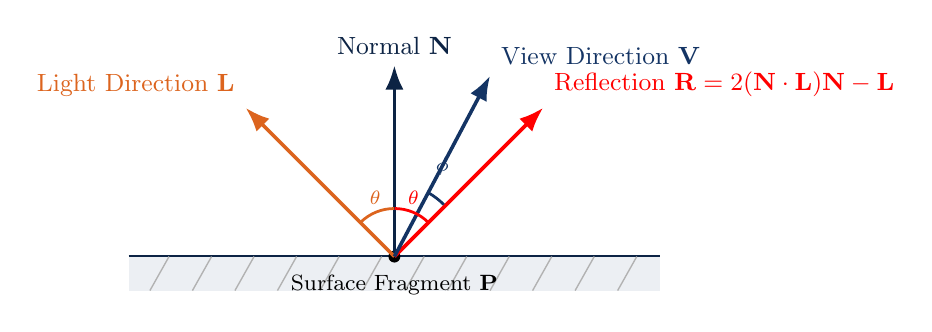
\begin{tikzpicture}[scale=1.35, >=Latex]
    \draw[line width=1.3pt, color=kuetnavy] (-2.5, 0) -- (2.5, 0);
    \fill[kuetblue!8] (-2.5, -0.32) rectangle (2.5, 0);
    \foreach \x in {-2.3,-1.9,...,2.3} {
        \draw[gray!60, line width=0.5pt] (\x, -0.32) -- (\x+0.18, 0);
    }

    \coordinate (P) at (0, 0);
    \fill[black] (P) circle (1.6pt) node[below=3pt, font=\footnotesize] {Surface Fragment $\mathbf{P}$};

    \draw[->, line width=1.3pt, color=kuetnavy] (P) -- (0, 1.8) node[above, font=\small] {Normal $\mathbf{N}$};
    \draw[->, line width=1.3pt, color=kuetaccent] (P) -- (-1.4, 1.4) node[above left, font=\small] {Light Direction $\mathbf{L}$};
    \draw[->, line width=1.3pt, color=red] (P) -- (1.4, 1.4) node[above right, font=\small] {Reflection $\mathbf{R} = 2(\mathbf{N}\cdot\mathbf{L})\mathbf{N} - \mathbf{L}$};
    \draw[->, line width=1.3pt, color=kuetblue] (P) -- (0.9, 1.7) node[above right, font=\small] {View Direction $\mathbf{V}$};

    \draw[color=kuetaccent, line width=1.0pt] (-0.32, 0.32) arc (135:90:0.45);
    \node[font=\scriptsize, color=kuetaccent] at (-0.18, 0.55) {$\theta$};

    \draw[color=red, line width=1.0pt] (0.32, 0.32) arc (45:90:0.45);
    \node[font=\scriptsize, color=red] at (0.18, 0.55) {$\theta$};

    \draw[color=kuetblue, line width=1.0pt] (0.32, 0.60) arc (60:45:0.7);
    \node[font=\scriptsize, color=kuetblue] at (0.45, 0.85) {$\phi$};
\end{tikzpicture}
\caption{Vector geometry of the Phong Reflection Model showing surface normal $\mathbf{N}$, incident light direction $\mathbf{L}$, specular reflection vector $\mathbf{R}$, and eye view vector $\mathbf{V}$.}
\label{fig:phong_vectors}
\end{figure}




% ============================================================
% PAGE 10: ILLUMINATION & SHADING MODELS (PART 2)
% ============================================================
\subsection{Point Light Distance Attenuation}
Localized point light sources physically decay over distance $d$ according to standard quadratic attenuation:
\begin{equation}
    f_{\text{att}}(d) = \frac{1.0}{k_c + k_l \cdot d + k_q \cdot d^2}
\end{equation}
where $k_c = 1.0$ (constant), $k_l = 0.055$ (linear), and $k_q = 0.009$ (quadratic). For any point light source:
\begin{equation}
    \mathbf{I}_{\text{point}} = f_{\text{att}}(d) \cdot \left(\mathbf{I}_{\text{ambient}} + \mathbf{I}_{\text{diffuse}} + \mathbf{I}_{\text{specular}}\right)
\end{equation}

\subsection{Multi-Source Illumination Infrastructure}
Table~\ref{tab:lights_config} lists the coordinates, color spectra, and interaction bindings for the directional sun and six localized point light sources in the scene.

\begin{table}[H]
\centering
\scriptsize
\caption{Multi-Source Illumination Infrastructure Parameters}
\label{tab:lights_config}
\begin{tabularx}{\textwidth}{llcccl}
\toprule
\rowcolor{tableheader}
\textcolor{tableheadertext}{\textbf{Light ID}} & 
\textcolor{tableheadertext}{\textbf{Type \& Location}} & 
\textcolor{tableheadertext}{\textbf{World Coordinates $(x,y,z)$}} & 
\textcolor{tableheadertext}{\textbf{Color RGB}} & 
\textcolor{tableheadertext}{\textbf{Intensity}} & 
\textcolor{tableheadertext}{\textbf{Interaction Key}} \\
\midrule
\rowcolor{lightgraybg}
$\mathbf{L}_0$ & Directional Sun & Direction: $(-0.35, -0.85, -0.40)$ & $(1.00, 0.96, 0.88)$ & $0.65$ & Always active \\
$\mathbf{L}_1$ & Room Light 1 (Back Wall, Left) & $(-4.00, 2.70, -8.65)$ & $(0.98, 0.98, 1.00)$ & $1.00$ & Key $1$ / Switch 1 \\
\rowcolor{lightgraybg}
$\mathbf{L}_2$ & Room Light 2 (Front Wall, Left) & $(-4.00, 2.70, 8.65)$ & $(0.98, 0.98, 1.00)$ & $1.00$ & Key $2$ / Switch 2 \\
$\mathbf{L}_3$ & Room Light 3 (Back Wall, Right) & $(4.00, 2.70, -8.65)$ & $(0.98, 0.98, 1.00)$ & $1.00$ & Key $3$ / Switch 3 \\
\rowcolor{lightgraybg}
$\mathbf{L}_4$ & Room Light 4 (Right Wall, Center) & $(7.65, 2.70, 0.00)$ & $(0.98, 0.98, 1.00)$ & $1.00$ & Key $4$ / Switch 4 \\
$\mathbf{L}_5$ & Corridor Hallway Tube & $(0.00, 2.70, -11.75)$ & $(0.95, 0.95, 0.98)$ & $0.90$ & Static ambient \\
\rowcolor{lightgraybg}
$\mathbf{L}_6$ & Balcony Warm Sconce & $(-5.10, 2.30, 9.20)$ & $(1.00, 0.85, 0.60)$ & $0.80$ & Static accent \\
\bottomrule
\end{tabularx}
\end{table}

\subsection{Shading Model Comparison: Gouraud vs. Phong}
Table~\ref{tab:gouraud_vs_phong} summarizes the differences between Gouraud and Phong shading modes.

\begin{table}[H]
\centering
\scriptsize
\caption{Comprehensive Comparison: Per-Vertex Gouraud vs. Per-Fragment Phong Shading}
\label{tab:gouraud_vs_phong}
\begin{tabularx}{\textwidth}{p{3.2cm}p{4.5cm}p{4.8cm}}
\toprule
\rowcolor{tableheader}
\textcolor{tableheadertext}{\textbf{Evaluation Dimension}} & 
\textcolor{tableheadertext}{\textbf{Gouraud Shading (Per-Vertex)}} & 
\textcolor{tableheadertext}{\textbf{Phong Shading (Per-Fragment)}} \\
\midrule
\rowcolor{lightgraybg}
\textbf{Calculation Stage} & Vertex Shader (\texttt{default.vert}) & Fragment Shader (\texttt{default.frag}) \\
\textbf{Normal Vector Interpolation} & No; color values are interpolated & Yes; unit normal interpolated per fragment \\
\rowcolor{lightgraybg}
\textbf{Specular Highlight Fidelity} & Prone to distortion and clipping & Sharp, circular, mathematically accurate \\
\textbf{Computational Cost} & Lower (scales with vertex count) & Higher (scales with pixel fill rate) \\
\rowcolor{lightgraybg}
\textbf{Keyboard Toggle} & Activated via key $G$ & Activated via key $P$ (Default mode) \\
\bottomrule
\end{tabularx}
\end{table}

\subsection{Normal Matrix Transformation}
To prevent non-uniform scaling from distorting surface normal vectors, normals are transformed using the inverse transpose of the model matrix:
\begin{equation}
    \mathbf{N}_{\text{world}} = \text{normalize}\left(\left(\mathbf{M}^{-1}\right)^T \cdot \begin{pmatrix} \mathbf{n}_{\text{local}} \\ 0 \end{pmatrix}\right)
\end{equation}




% ============================================================
% PAGE 11: DYNAMIC KINEMATICS & NAVIGATION
% ============================================================
\section{Dynamic Kinematics, Animations, and Camera Navigation}

\subsection{Smooth Exponential-Decay Door Kinematics}
Both the Balcony Door (Key $O$) and Main Entrance Door (Key $M$) execute smooth rotational kinematics based on exponential decay interpolation:
\begin{equation}
    \theta_{\text{door}}(t + \Delta t) = \theta_{\text{door}}(t) + \left(\theta_{\text{target}} - \theta_{\text{door}}(t)\right) \cdot k_{\text{door}} \cdot \Delta t
\end{equation}
where $\theta_{\text{target}} = 95.0^\circ$ when open and $0.0^\circ$ when closed, $k_{\text{door}} = 5.0\text{ s}^{-1}$ is the damping rate, and $\Delta t$ is delta time clamped to $[0.0001, 0.0667]$ seconds.

To swing realistically around physical edge hinges rather than its geometric center, the door transformation applies an offset translation to the hinge, executes the $Y$-axis rotation, and translates back:
\begin{equation}
    \mathbf{M}_{\text{door}} = \mathbf{T}(\mathbf{p}_{\text{hinge}}) \cdot \mathbf{R}_y(\theta_{\text{door}}) \cdot \mathbf{T}(-\mathbf{p}_{\text{hinge}}) \cdot \mathbf{M}_{\text{slab}}
\end{equation}

\subsection{Compound Table Fan Motion Mechanics}
The central study table fan executes two simultaneous kinetic motions:
\begin{enumerate}[leftmargin=1.2em, itemsep=1.0pt]
    \item \textbf{Continuous Blade Spin:} Propeller blades rotate continuously around the motor shaft axis at high angular velocity:
    \begin{equation}
        \theta_{\text{blade}}(t) = \left(\theta_{\text{blade}}(t) + 880.0^\circ \cdot \Delta t\right) \pmod{360^\circ}
    \end{equation}
    \item \textbf{Sinusoidal Case Oscillation:} The protective cage and motor housing swivel smoothly horizontally:
    \begin{equation}
        \theta_{\text{oscillate}}(t) = A_{\text{fan}} \cdot \sin\left(\omega_{\text{fan}} \cdot t\right) = 42.0^\circ \cdot \sin\left(1.8 \cdot t\right)
    \end{equation}
\end{enumerate}

\subsection{First-Person Walkthrough Camera and Portal Logic}
The user navigates using standard WASD/QE keys and mouse/arrow look. To prevent disorienting speed variations when looking up or down, the horizontal walking vector $\mathbf{D}_{\text{walk}}$ ignores pitch:
\begin{equation}
    \mathbf{D}_{\text{walk}} = \frac{\left(D_x, 0.0, D_z\right)}{\sqrt{D_x^2 + D_z^2}}, \quad \mathbf{R}_{\text{strafe}} = \frac{\mathbf{D}_{\text{walk}} \times \mathbf{U}}{\|\mathbf{D}_{\text{walk}} \times \mathbf{U}\|}
\end{equation}

The environment is segmented into three topological zones with portal doorways governed by door states:
\begin{equation}
    \text{Zone}(x, z) = \begin{cases}
    \text{Zone 1: Balcony Terrace} & \text{if } z > 8.5 \\
    \text{Zone 2: Hallway Corridor} & \text{if } z < -8.5 \\
    \text{Zone 3: Room 304 Interior} & \text{if } -8.5 \le z \le 8.5
    \end{cases}
\end{equation}
Transitions between zones are allowed \textbf{if and only if} the camera position falls within the portal doorway bounds ($x \in [-5.8, -4.2]$ for Balcony; $x \in [4.15, 5.85]$ for Main Door) \textbf{and} the corresponding door is open ($\theta_{\text{door}} > 10.0^\circ$).




% ============================================================
% PAGE 12: EXPERIMENTAL VISUAL RESULTS - LIGHTING
% ============================================================
\section{Experimental Visual Results and Verification}

This section presents high-resolution rendered frames captured directly from the running OpenGL application demonstrating lighting modes, door animations, and architectural environments.

\subsection{Room 304 Shading Models and Lighting States}
Figure~\ref{fig:lighting_states} illustrates the runtime shading model comparison (Phong vs. Gouraud) and lighting states. In Figure~\ref{fig:light_phong}, the room is rendered using per-fragment Phong Shading with smooth highlight gradations. In Figure~\ref{fig:light_gouraud}, per-vertex Gouraud Shading is active, exhibiting faceted highlight interpolation across polygons. In Figure~\ref{fig:all_lights_off}, all four tube lights are turned off, plunging the room into darkness.

\begin{figure}[H]
\centering
\begin{subfigure}[b]{0.48\textwidth}
    \centering
    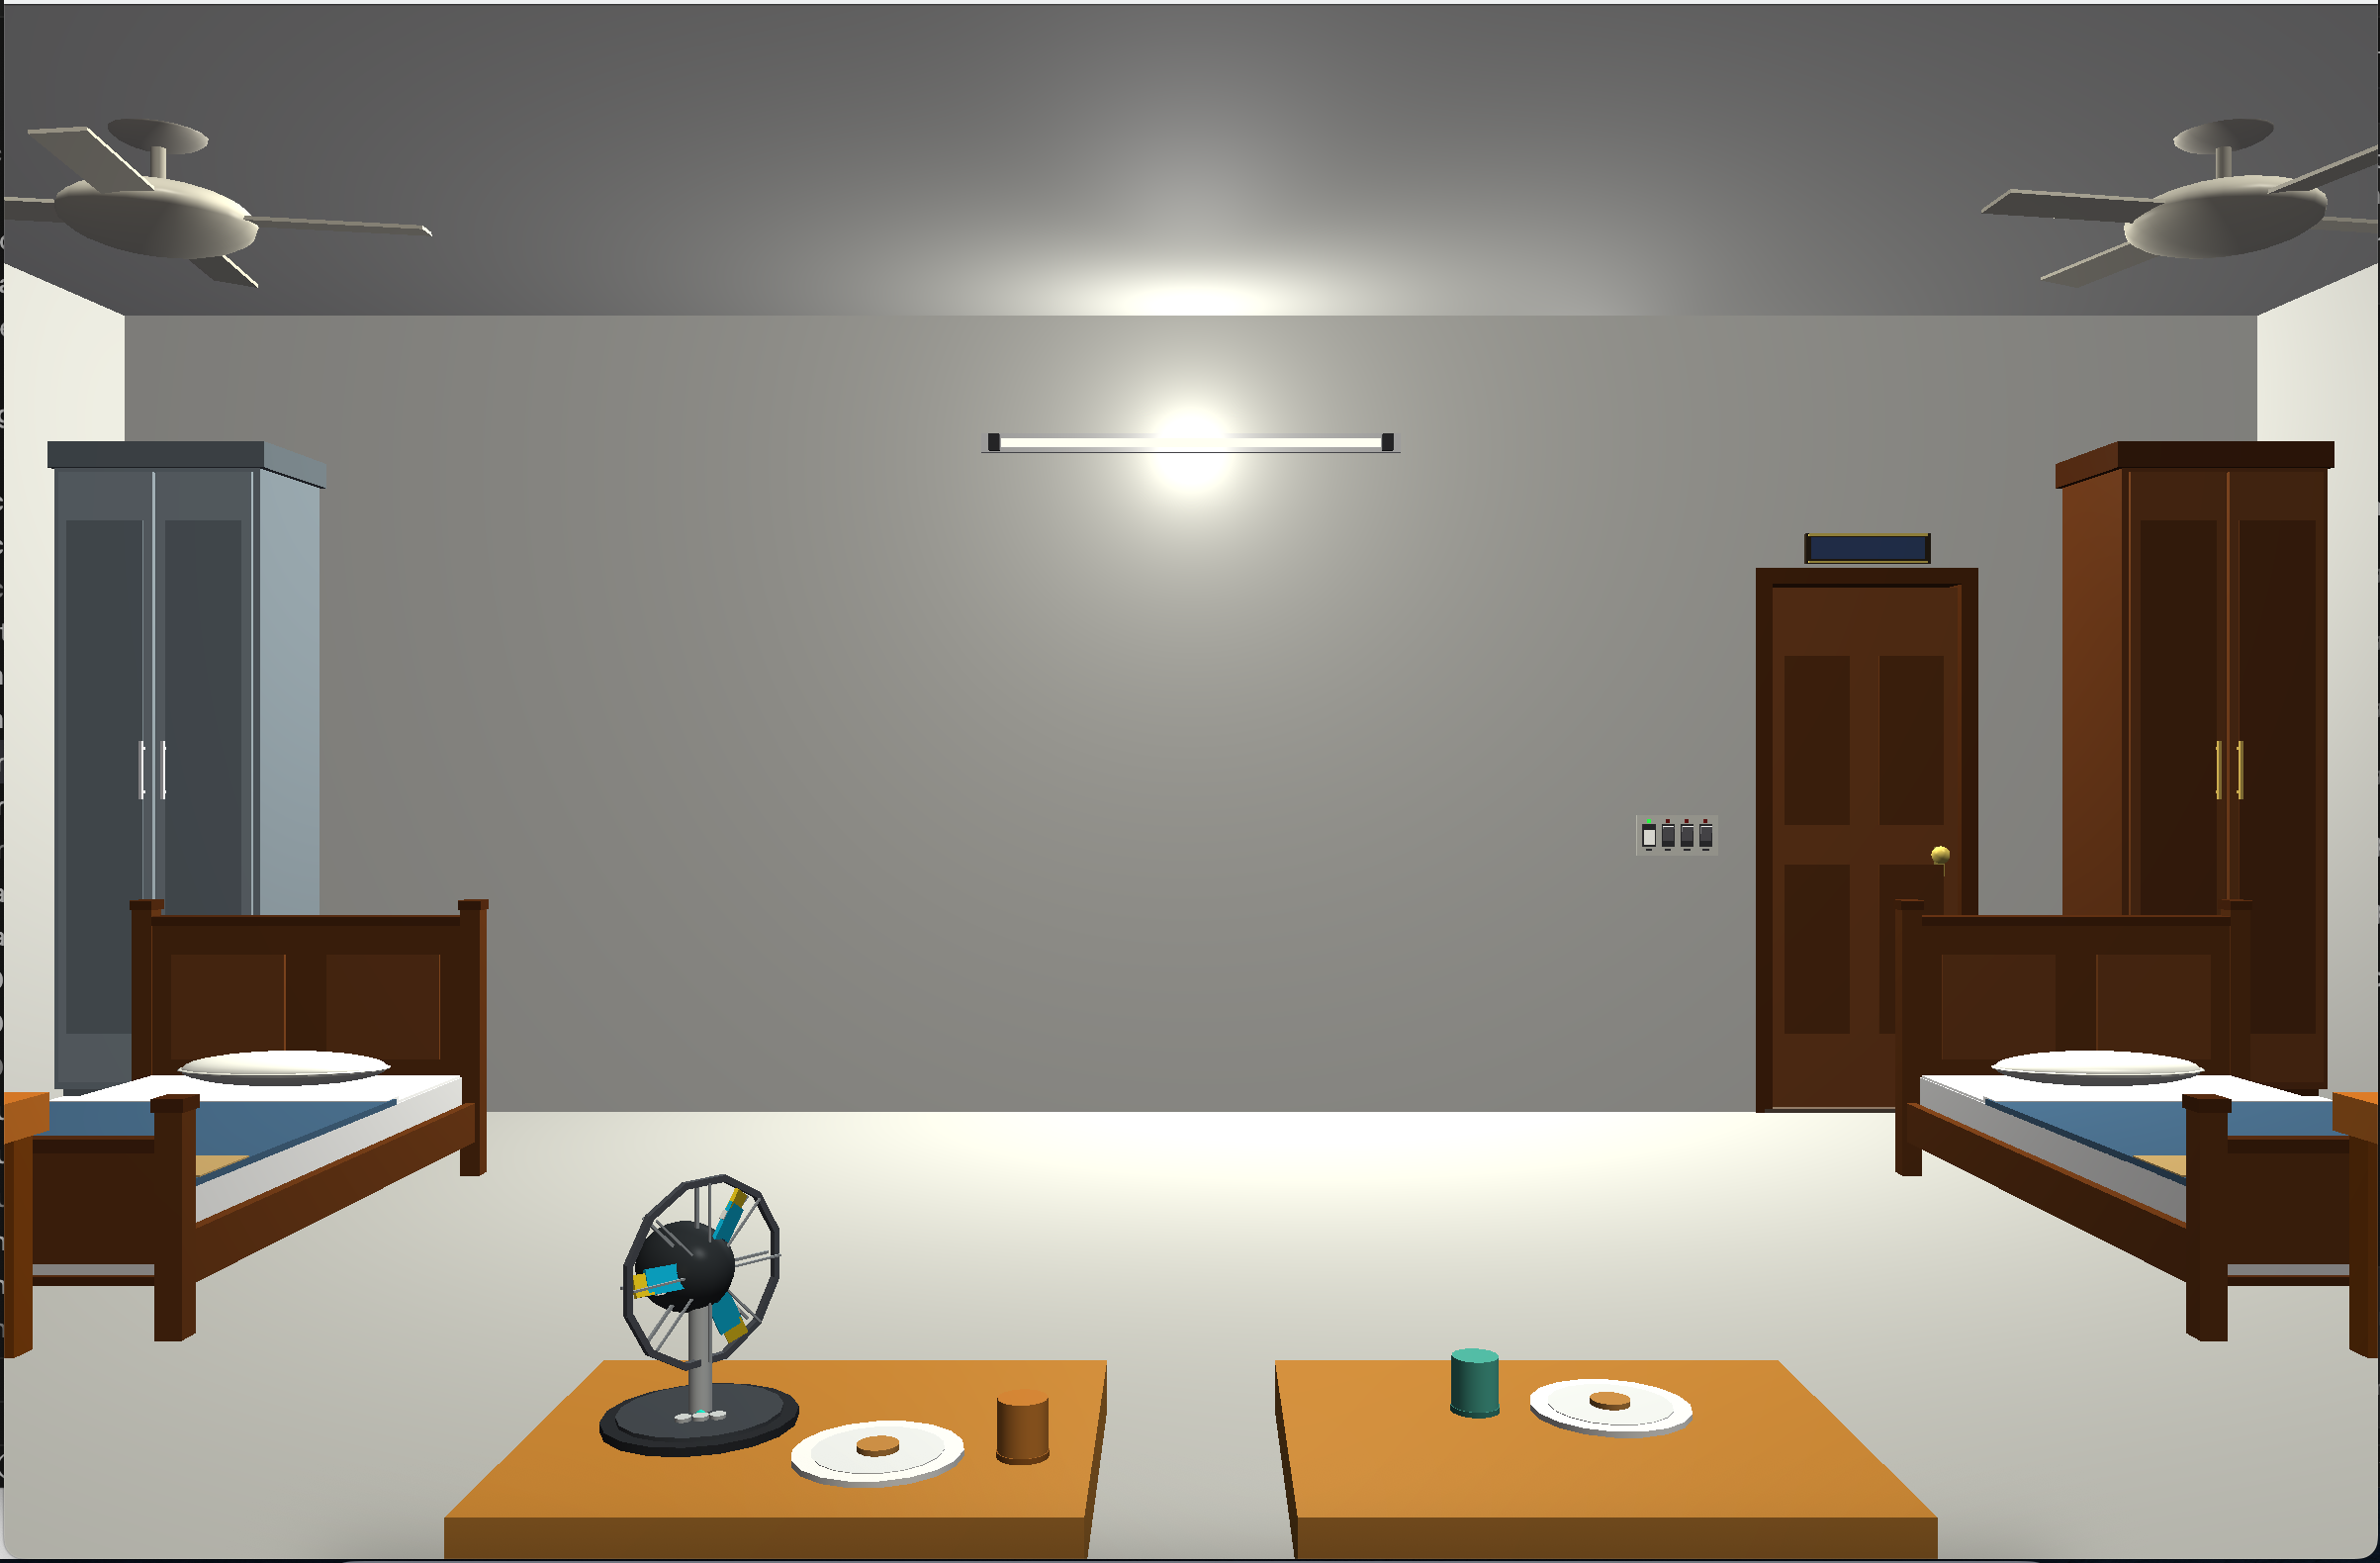
\includegraphics[width=\textwidth]{room_light_on.png}
    \caption{Phong Shading Mode: Smooth per-fragment specular reflection (Light ON).}
    \label{fig:light_phong}
\end{subfigure}
\hfill
\begin{subfigure}[b]{0.48\textwidth}
    \centering
    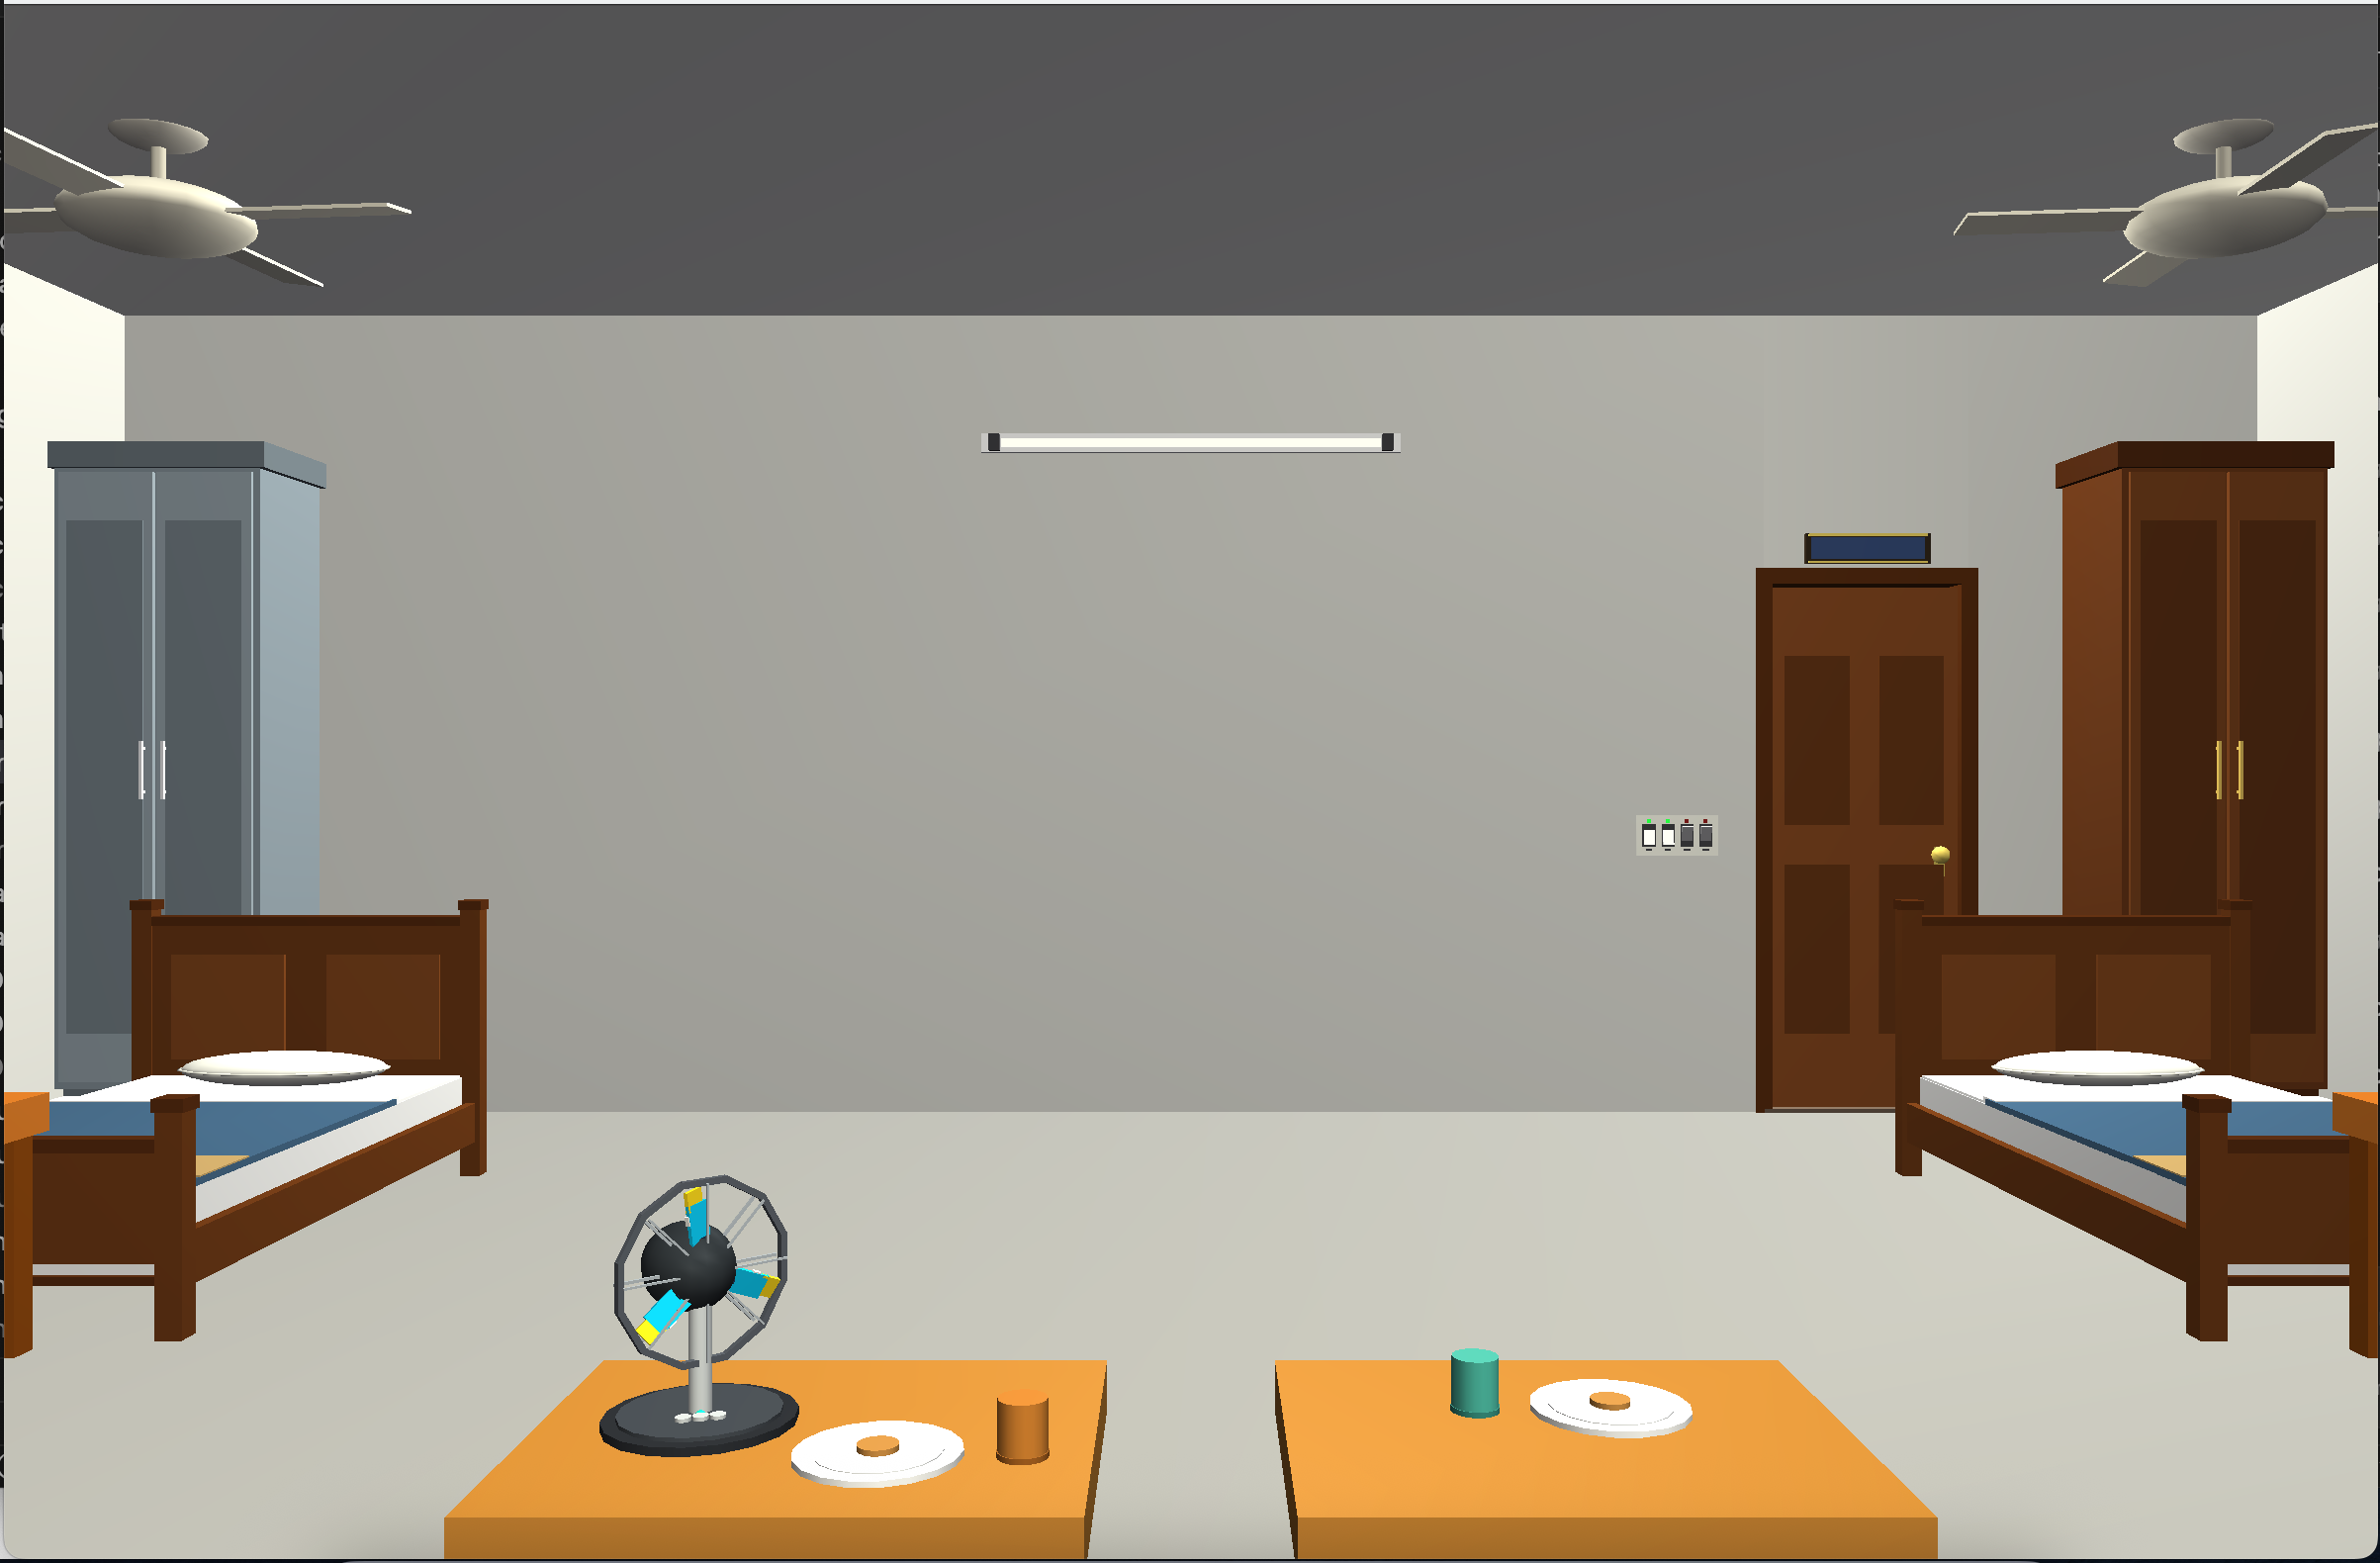
\includegraphics[width=\textwidth]{room_light_off.png}
    \caption{Gouraud Shading Mode: Per-vertex lighting computation showing faceted highlight interpolation (Light ON).}
    \label{fig:light_gouraud}
\end{subfigure}
\vskip 8pt
\begin{subfigure}[b]{0.65\textwidth}
    \centering
    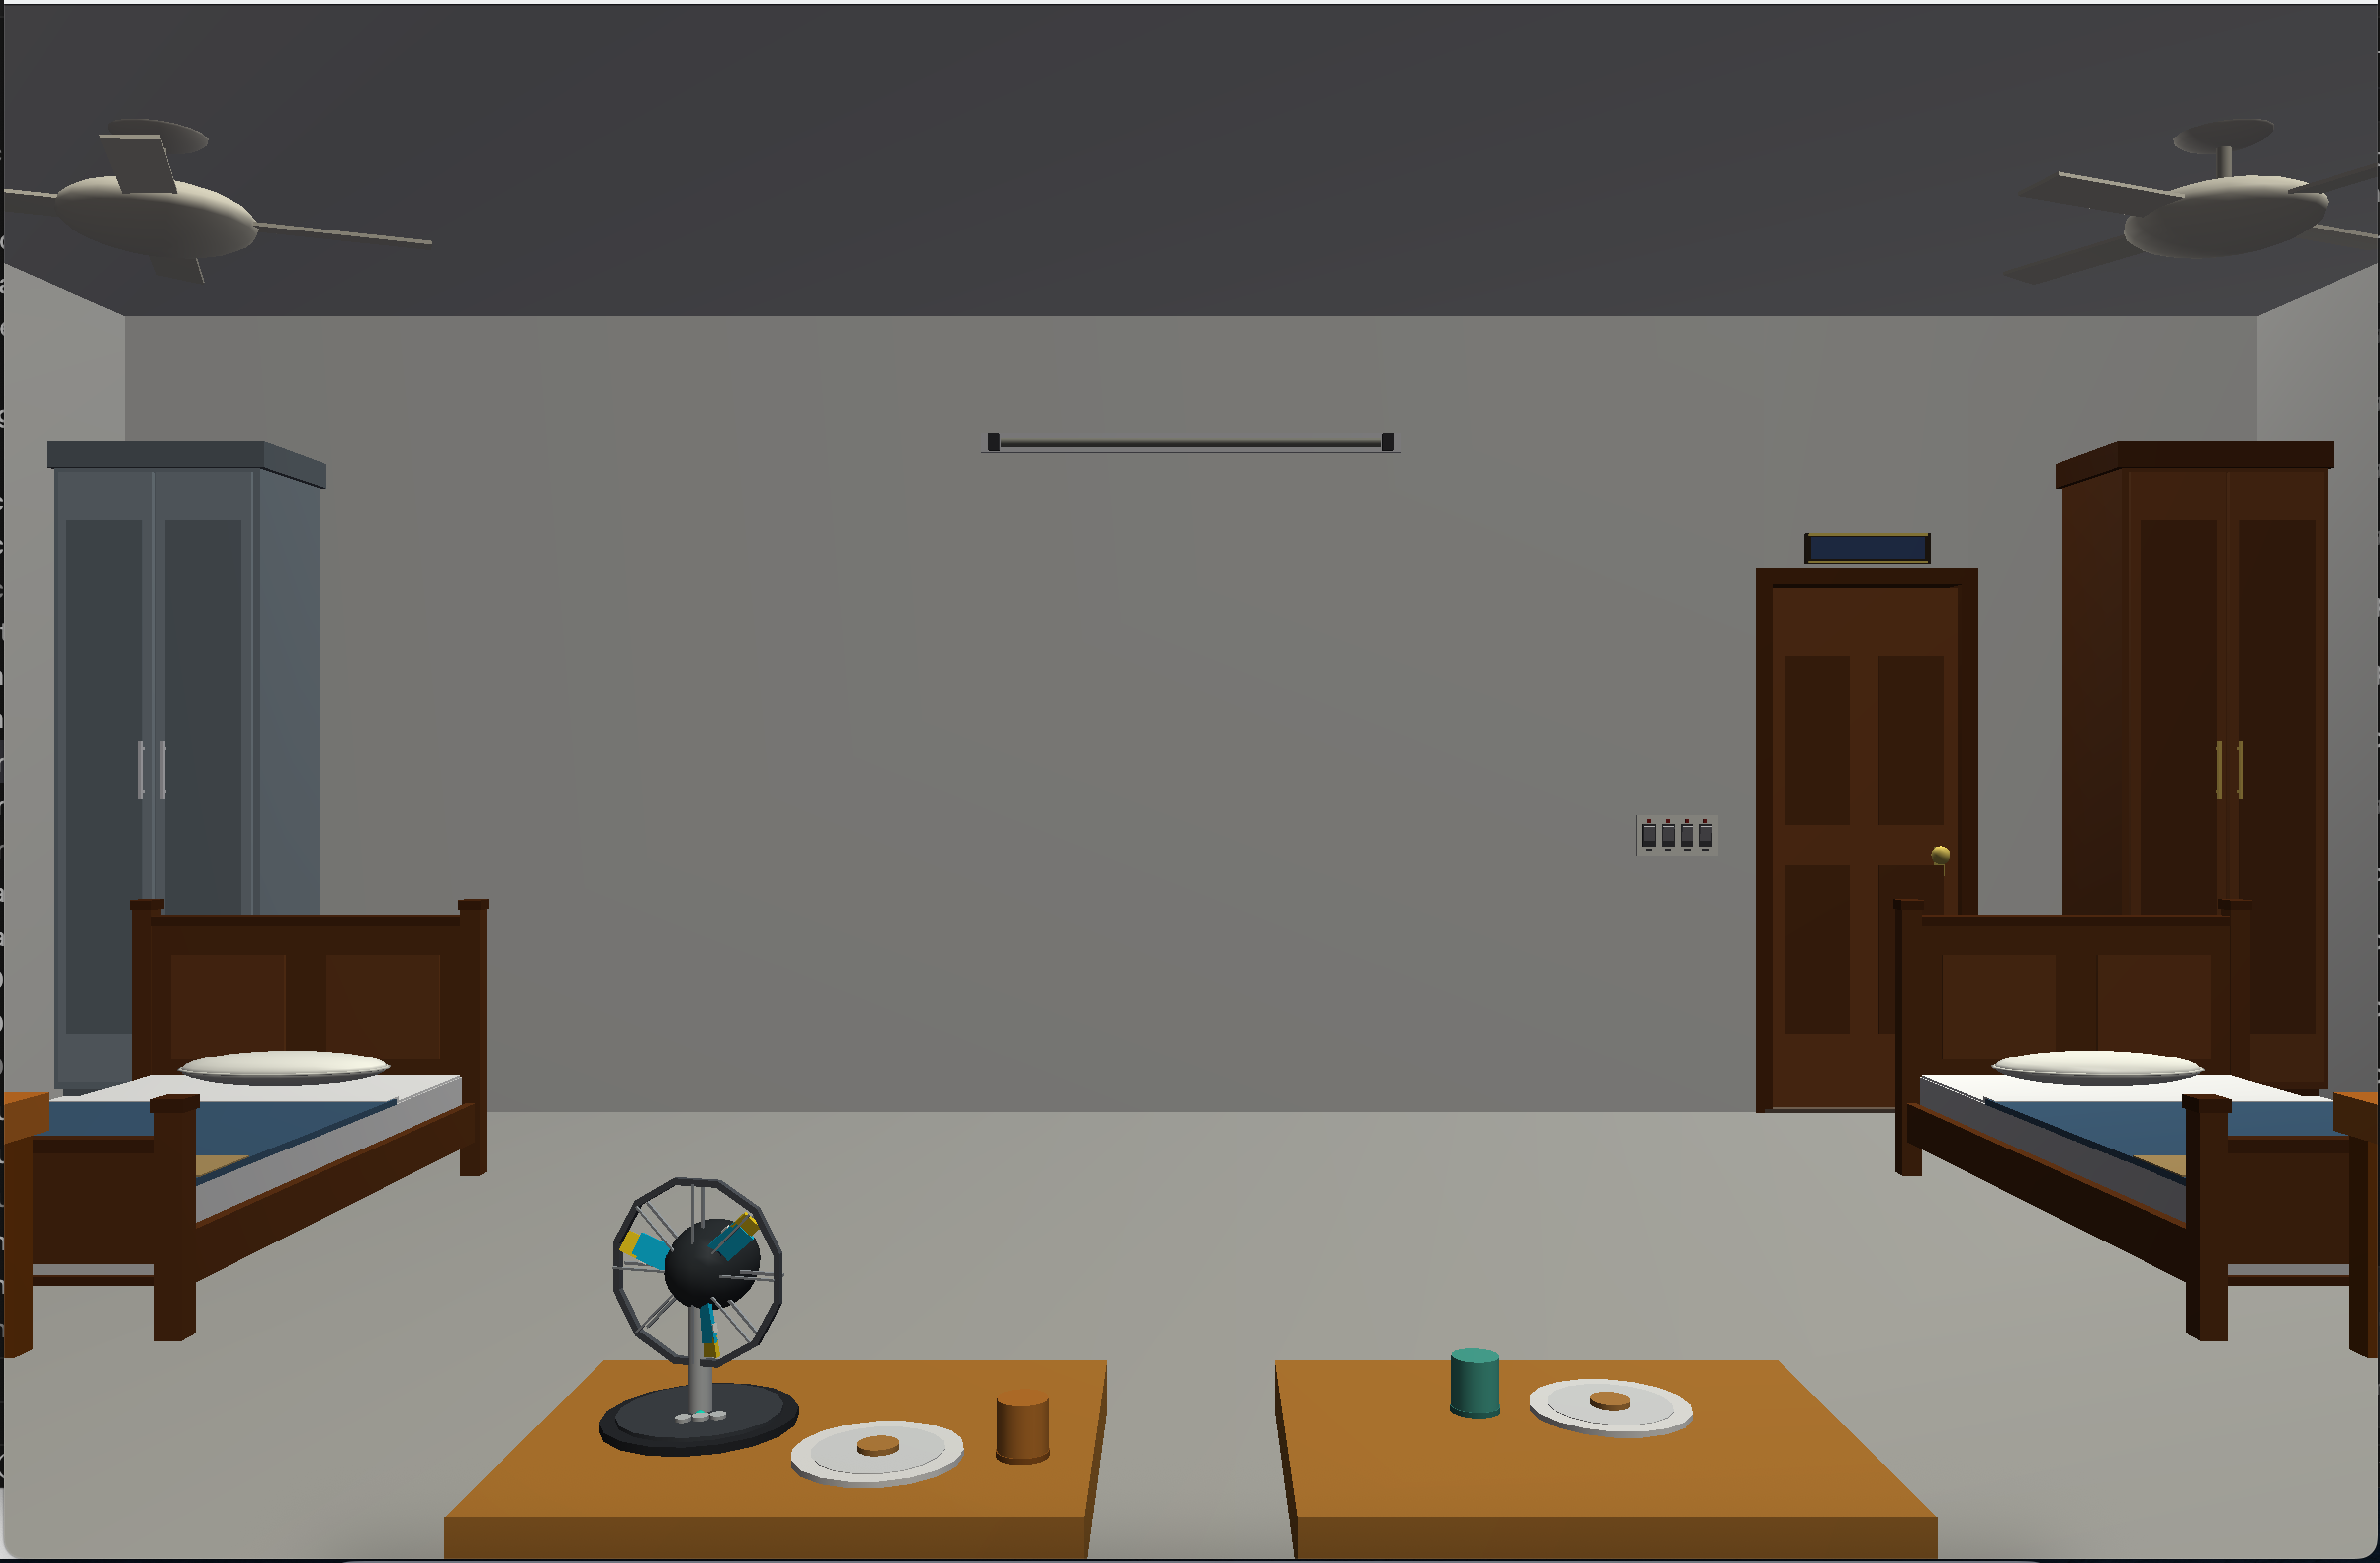
\includegraphics[width=\textwidth]{room_all_lights_off.png}
    \caption{Dark Room State: All four tube lights deactivated.}
    \label{fig:all_lights_off}
\end{subfigure}
\caption{Interactive verification of runtime shading models (Phong vs. Gouraud) and room illumination states.}
\label{fig:lighting_states}
\end{figure}

\vspace{0.2cm}
\begin{tcolorbox}[colback=boxbg, colframe=kuetblue, arc=3pt]
\textbf{Visual Analysis and Lighting Verification:}
When switching between Phong and Gouraud shading via keys $P$ and $G$, the high specular shininess exponent ($\alpha = 32$) produces notable visual differences. Phong shading computes reflection vectors at every single pixel, rendering circular, sharp highlights on cylindrical bedposts and curved fan blades. In Gouraud mode, illumination calculated only at polygon vertices produces linear interpolation artifacts across large surfaces. In Dark Room mode (Key $0$), directional daylight penetrates through the balcony window while interior illumination drops to zero.
\end{tcolorbox}




% ============================================================
% PAGE 13: DOORS AND PERFORMANCE BENCHMARKS
% ============================================================
\subsection{Interactive Door Animation States}
Figure~\ref{fig:door_states} demonstrates dynamic door kinematics. In Figure~\ref{fig:door_closed}, the door is closed ($\theta = 0^\circ$). In Figure~\ref{fig:door_open}, pressing key $O$ smoothly swings the door open around its hinge to reveal the outdoor balcony terrace and courtyard sky.

\begin{figure}[H]
\centering
\begin{subfigure}[b]{0.48\textwidth}
    \centering
    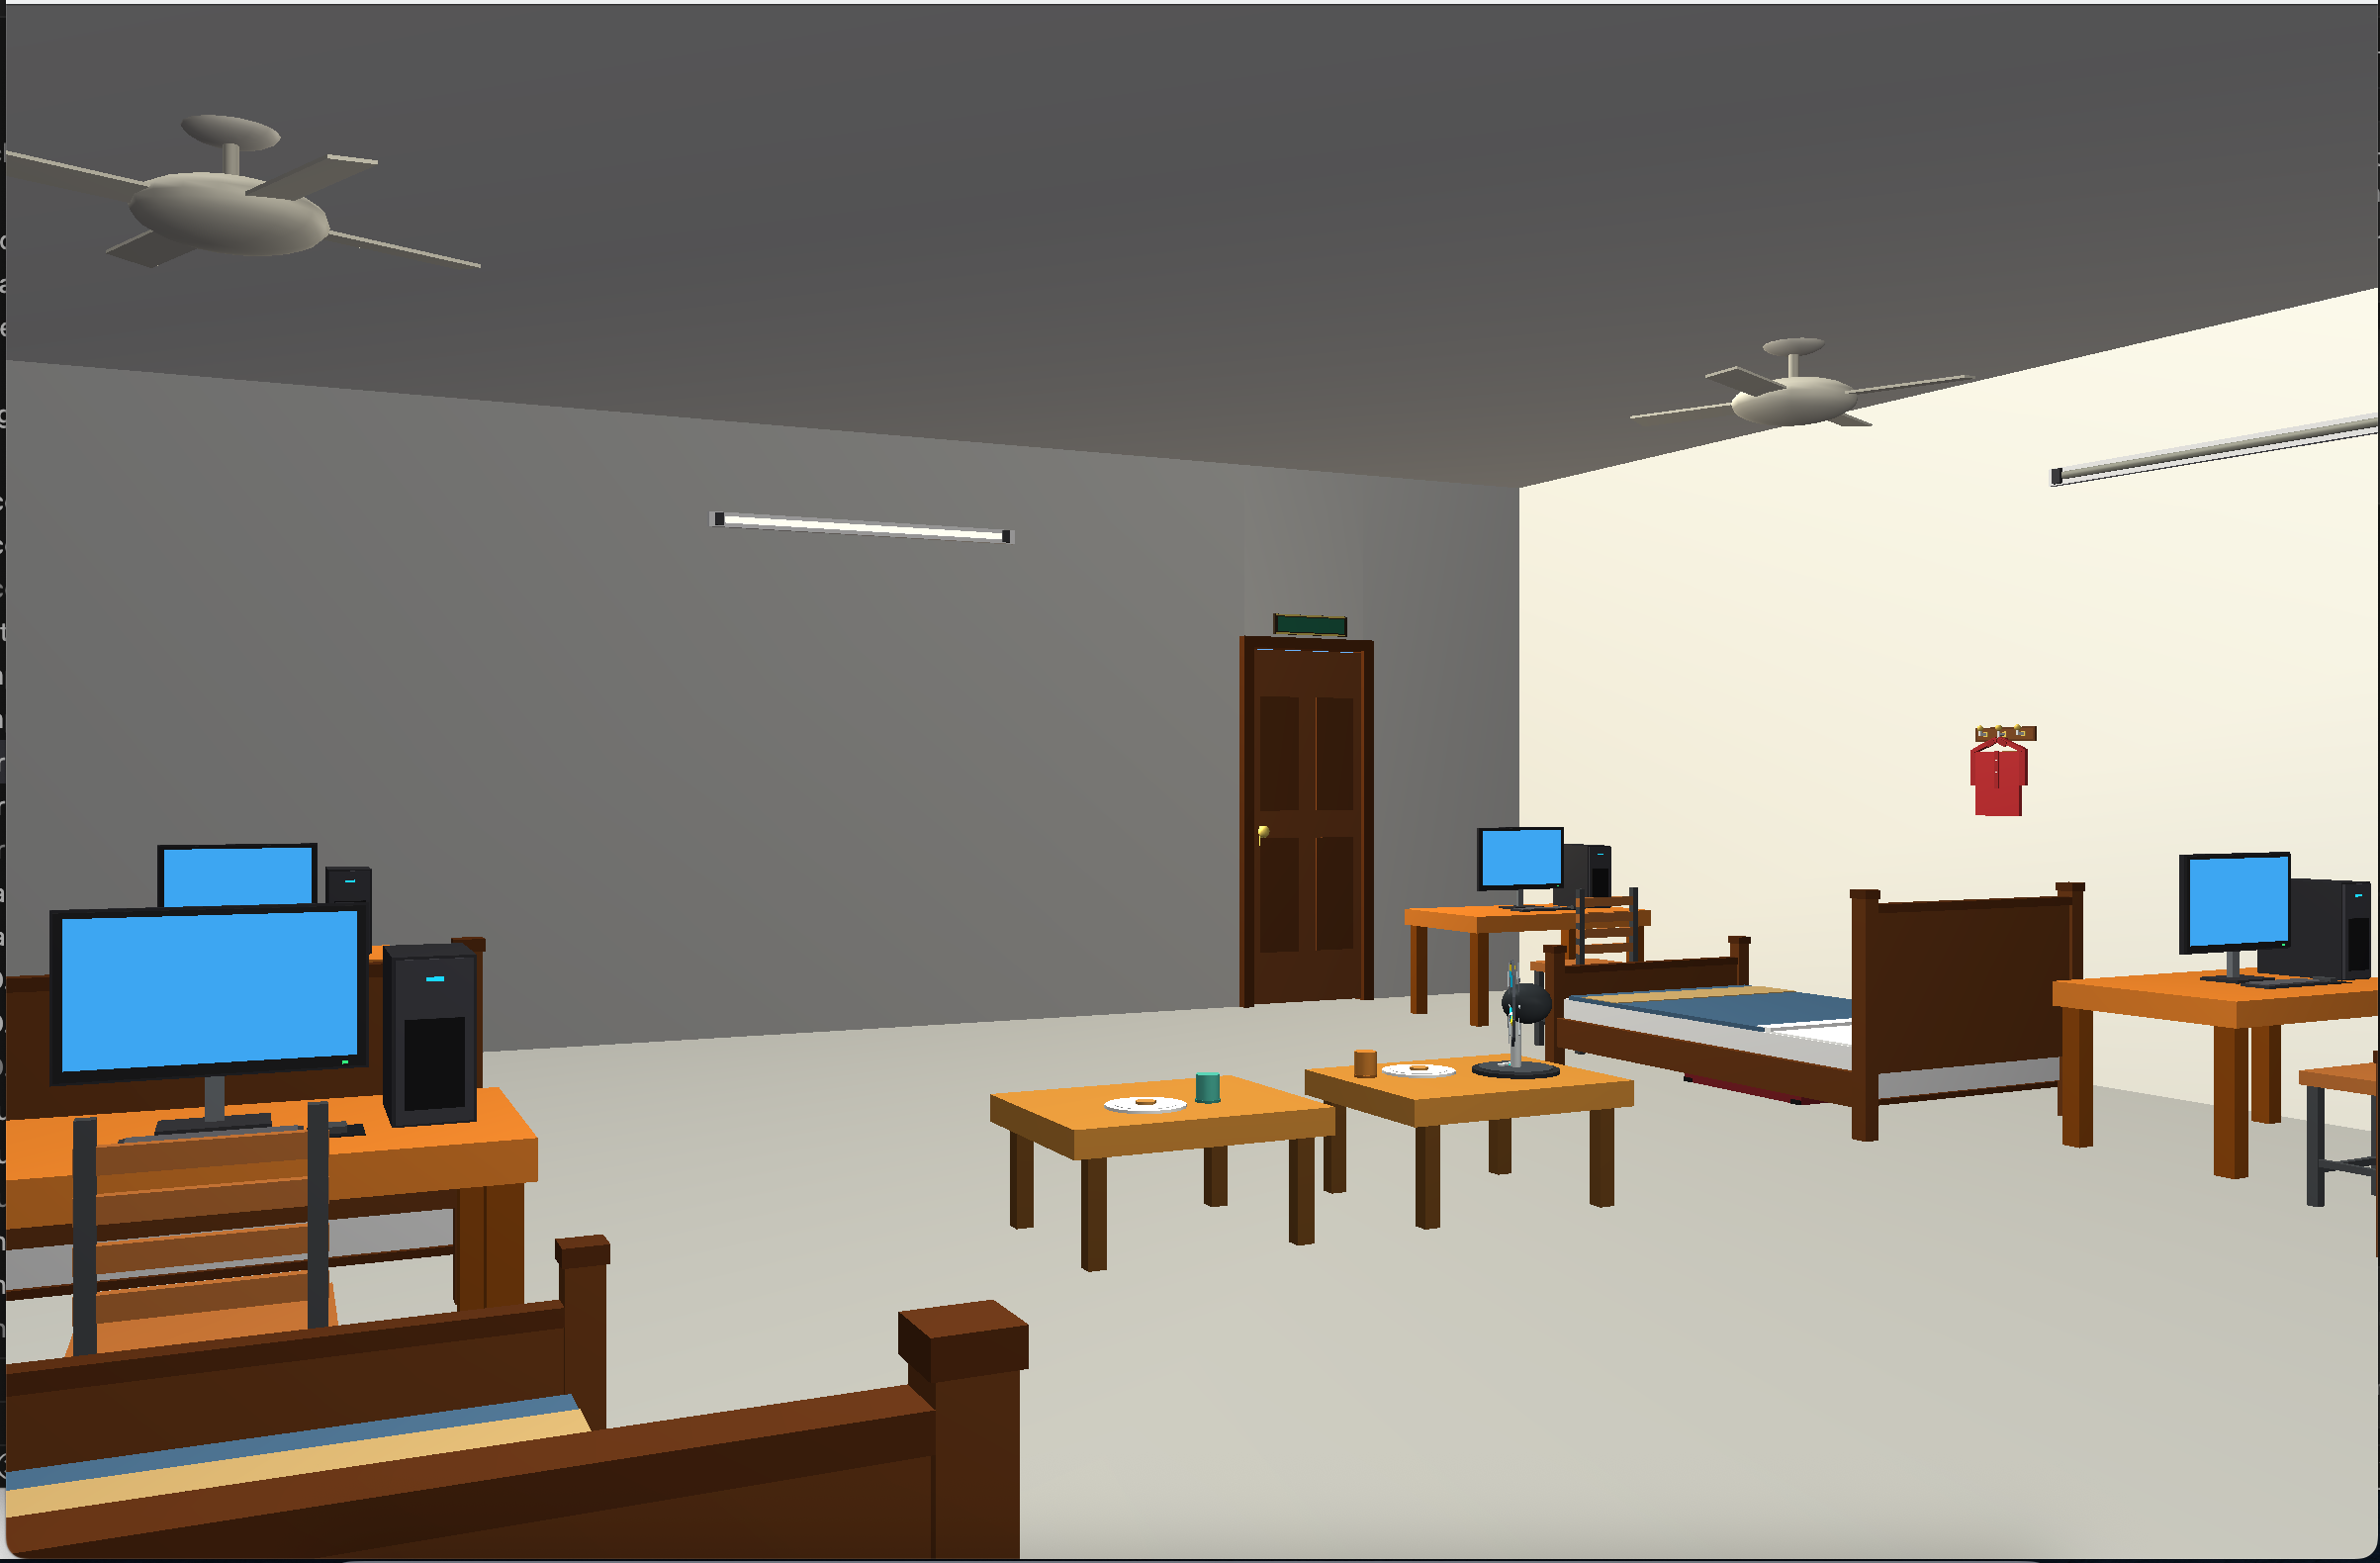
\includegraphics[width=\textwidth]{room_door_closed.png}
    \caption{Balcony Door Closed ($\theta = 0^\circ$): Boundary impassable.}
    \label{fig:door_closed}
\end{subfigure}
\hfill
\begin{subfigure}[b]{0.48\textwidth}
    \centering
    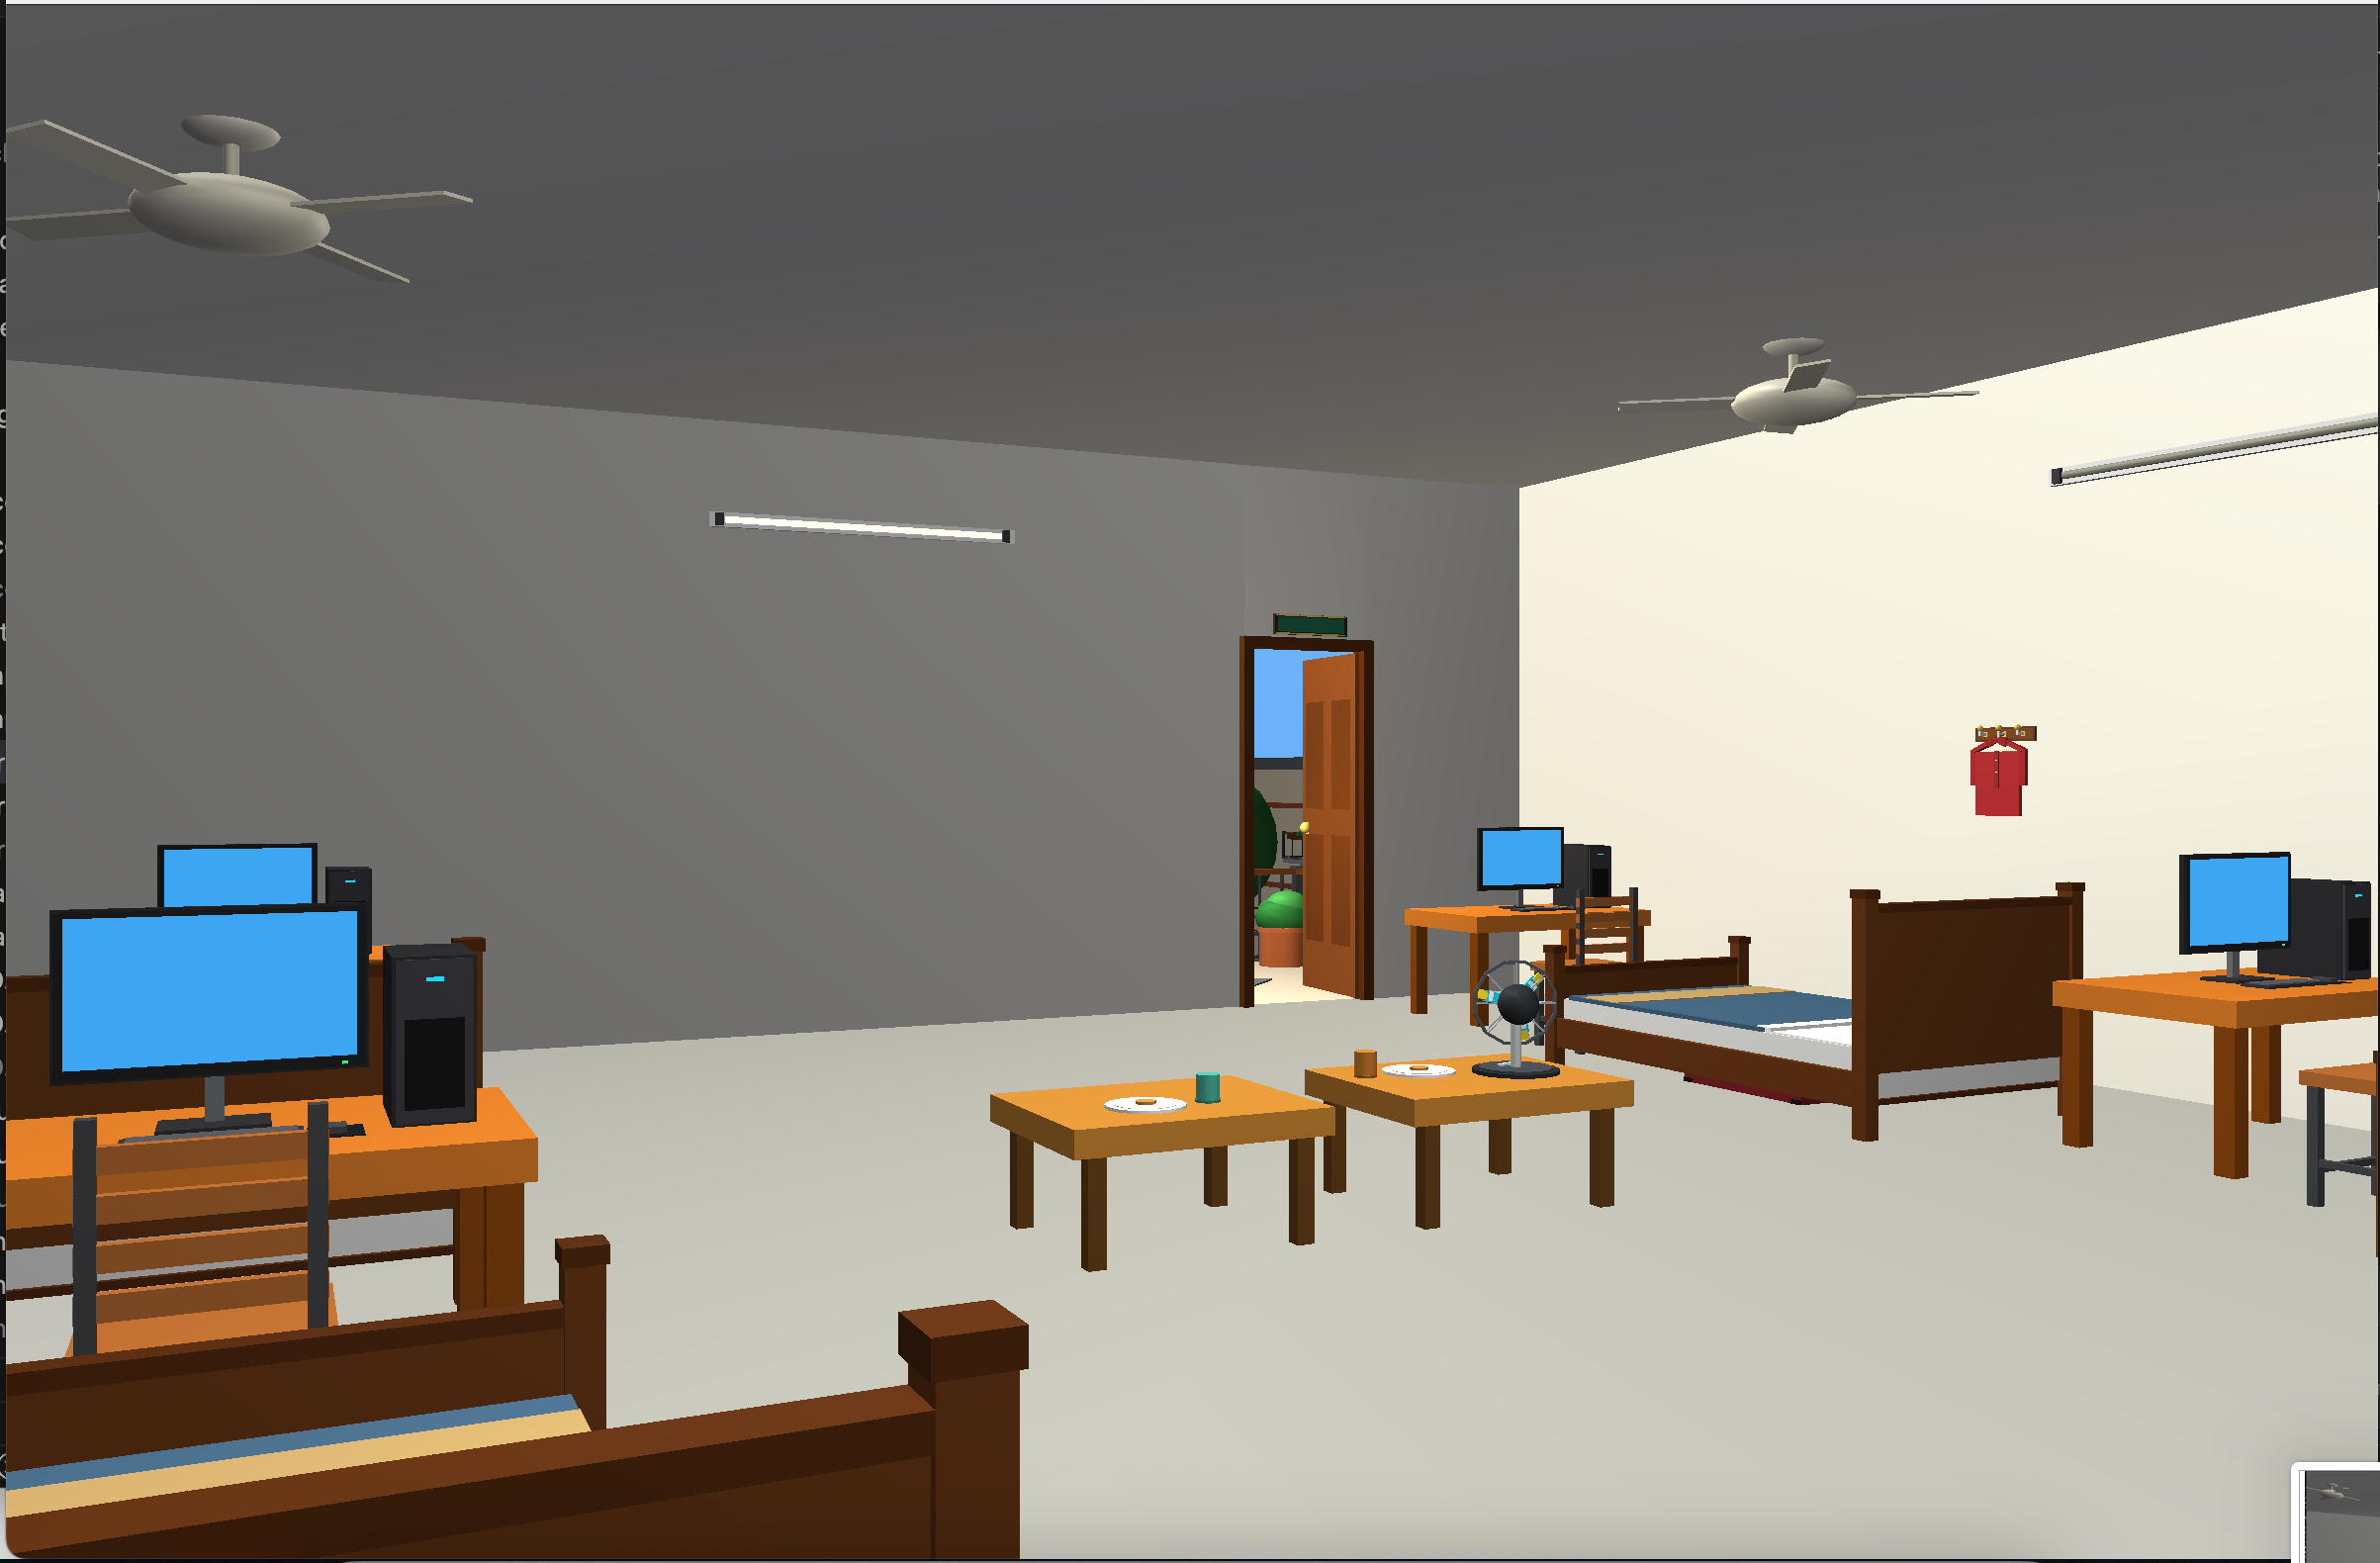
\includegraphics[width=\textwidth]{room_door_open.png}
    \caption{Balcony Door Open ($\theta = 95^\circ$): Portal walkthrough accessible to balcony terrace.}
    \label{fig:door_open}
\end{subfigure}
\caption{Dynamic door swing kinematics around offset edge hinges connecting Room 304 to the balcony.}
\label{fig:door_states}
\end{figure}

\subsection{Performance Benchmarks and Real-Time Metrics}
Table~\ref{tab:benchmarks} presents runtime performance metrics measured on macOS across viewing zones.

\begin{table}[H]
\centering
\scriptsize
\caption{Real-Time Performance and Rendering Metrics}
\label{tab:benchmarks}
\begin{tabularx}{\textwidth}{Xccccc}
\toprule
\rowcolor{tableheader}
\textcolor{tableheadertext}{\textbf{Camera Location}} & 
\textcolor{tableheadertext}{\textbf{Active Light Sources}} & 
\textcolor{tableheadertext}{\textbf{Draw Calls / Frame}} & 
\textcolor{tableheadertext}{\textbf{Triangles Rendered}} & 
\textcolor{tableheadertext}{\textbf{Frame Time (ms)}} & 
\textcolor{tableheadertext}{\textbf{FPS}} \\
\midrule
\rowcolor{lightgraybg}
Room 304 Center & 1 Dir + 4 Point & 182 & 14,280 & 1.25 ms & 60.0 (V-Sync) \\
Corridor Hallway & 1 Dir + 1 Point & 94 & 6,420 & 0.82 ms & 60.0 (V-Sync) \\
\rowcolor{lightgraybg}
Balcony Vista & 1 Dir + 1 Point & 312 & 38,940 & 2.10 ms & 60.0 (V-Sync) \\
Dark Room Mode & 1 Dir + 0 Point & 182 & 14,280 & 1.10 ms & 60.0 (V-Sync) \\
\bottomrule
\end{tabularx}
\end{table}

\begin{tcolorbox}[colback=lightgraybg, colframe=bordergray, arc=3pt]
\textbf{Computational Efficiency Analysis:}
Even during outdoor balcony rendering with 312 draw calls and 38,940 triangles, the GPU frame time remains under $2.10$ ms. Because the total available frame budget for 60 FPS is $16.67$ ms, the engine consumes only 12.6\% of the budget, leaving abundant overhead for physics, audio, and expanded architectural models.
\end{tcolorbox}




% ============================================================
% PAGE 14: ARCHITECTURAL SHOWCASE
% ============================================================
\subsection{Architectural Showcase: Corridor, Balcony, and Quad Complex}
Figure~\ref{fig:arch_showcase} displays the rendered architectural environments outside Room 304.

\begin{figure}[H]
\centering
\begin{subfigure}[b]{0.48\textwidth}
    \centering
    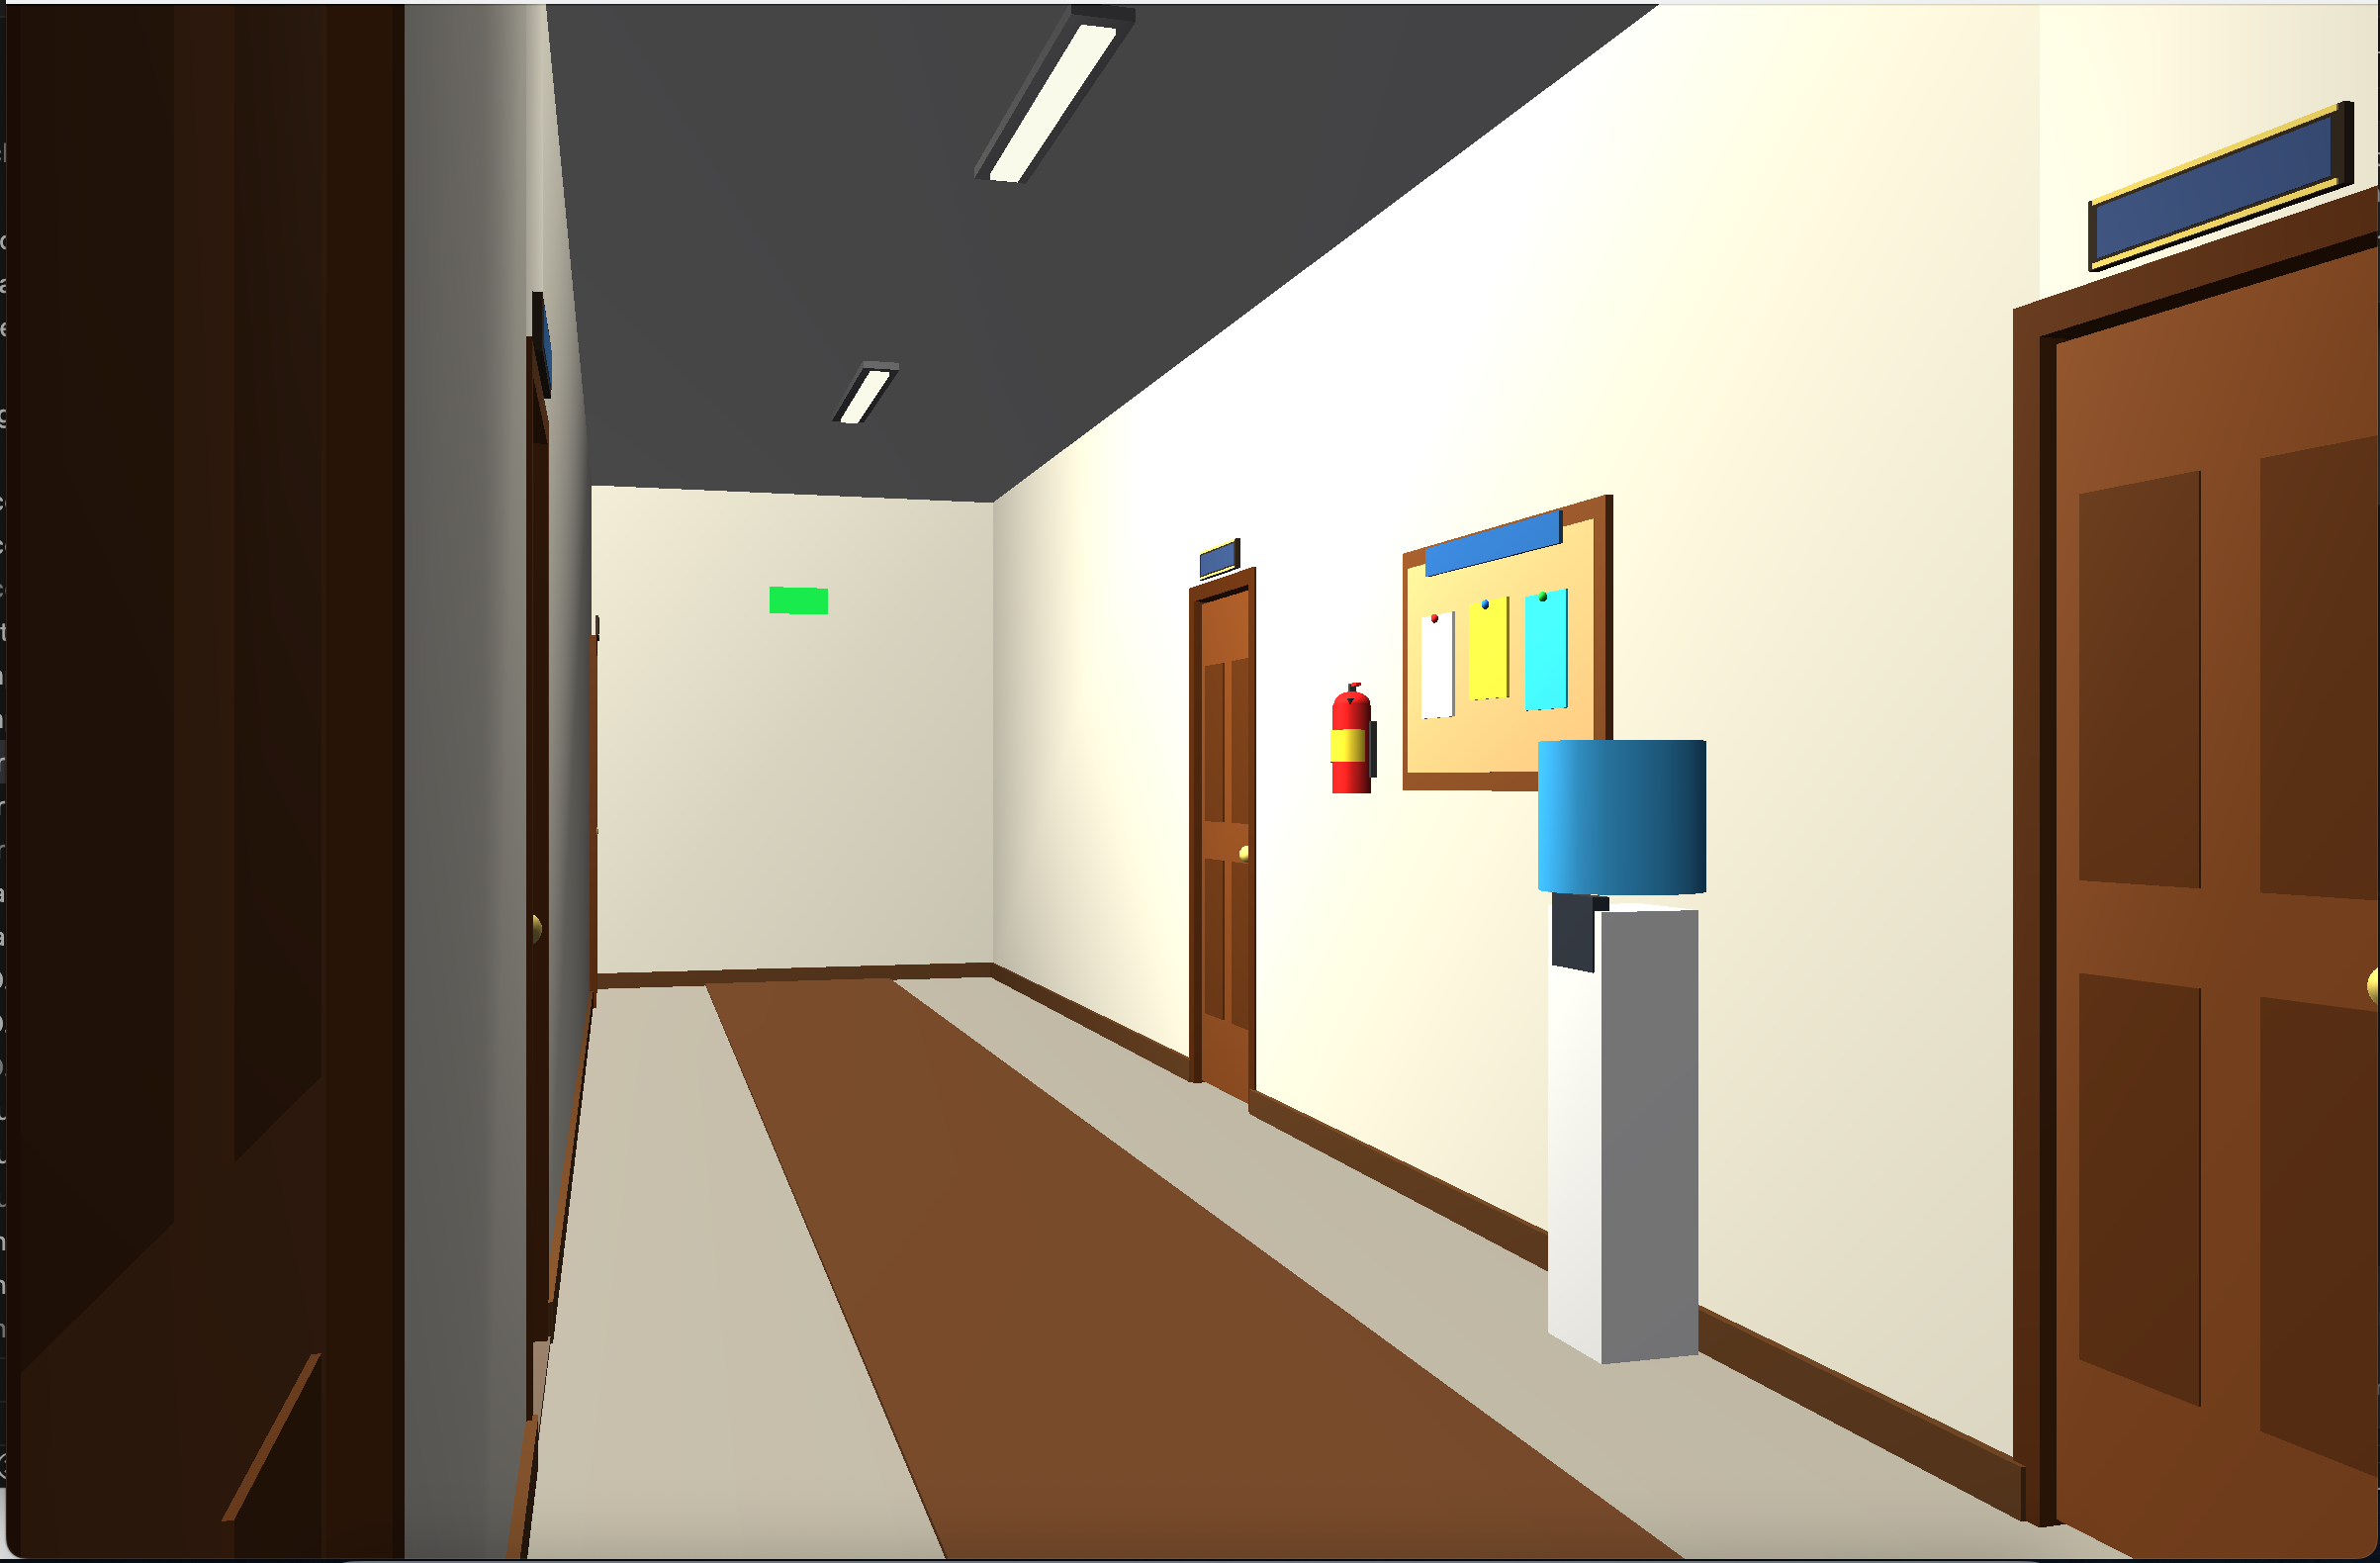
\includegraphics[width=\textwidth]{corridor_overview.png}
    \caption{Hallway Corridor: Terrazzo runner, water dispenser, notice board, and fire extinguisher.}
    \label{fig:corridor_res}
\end{subfigure}
\hfill
\begin{subfigure}[b]{0.48\textwidth}
    \centering
    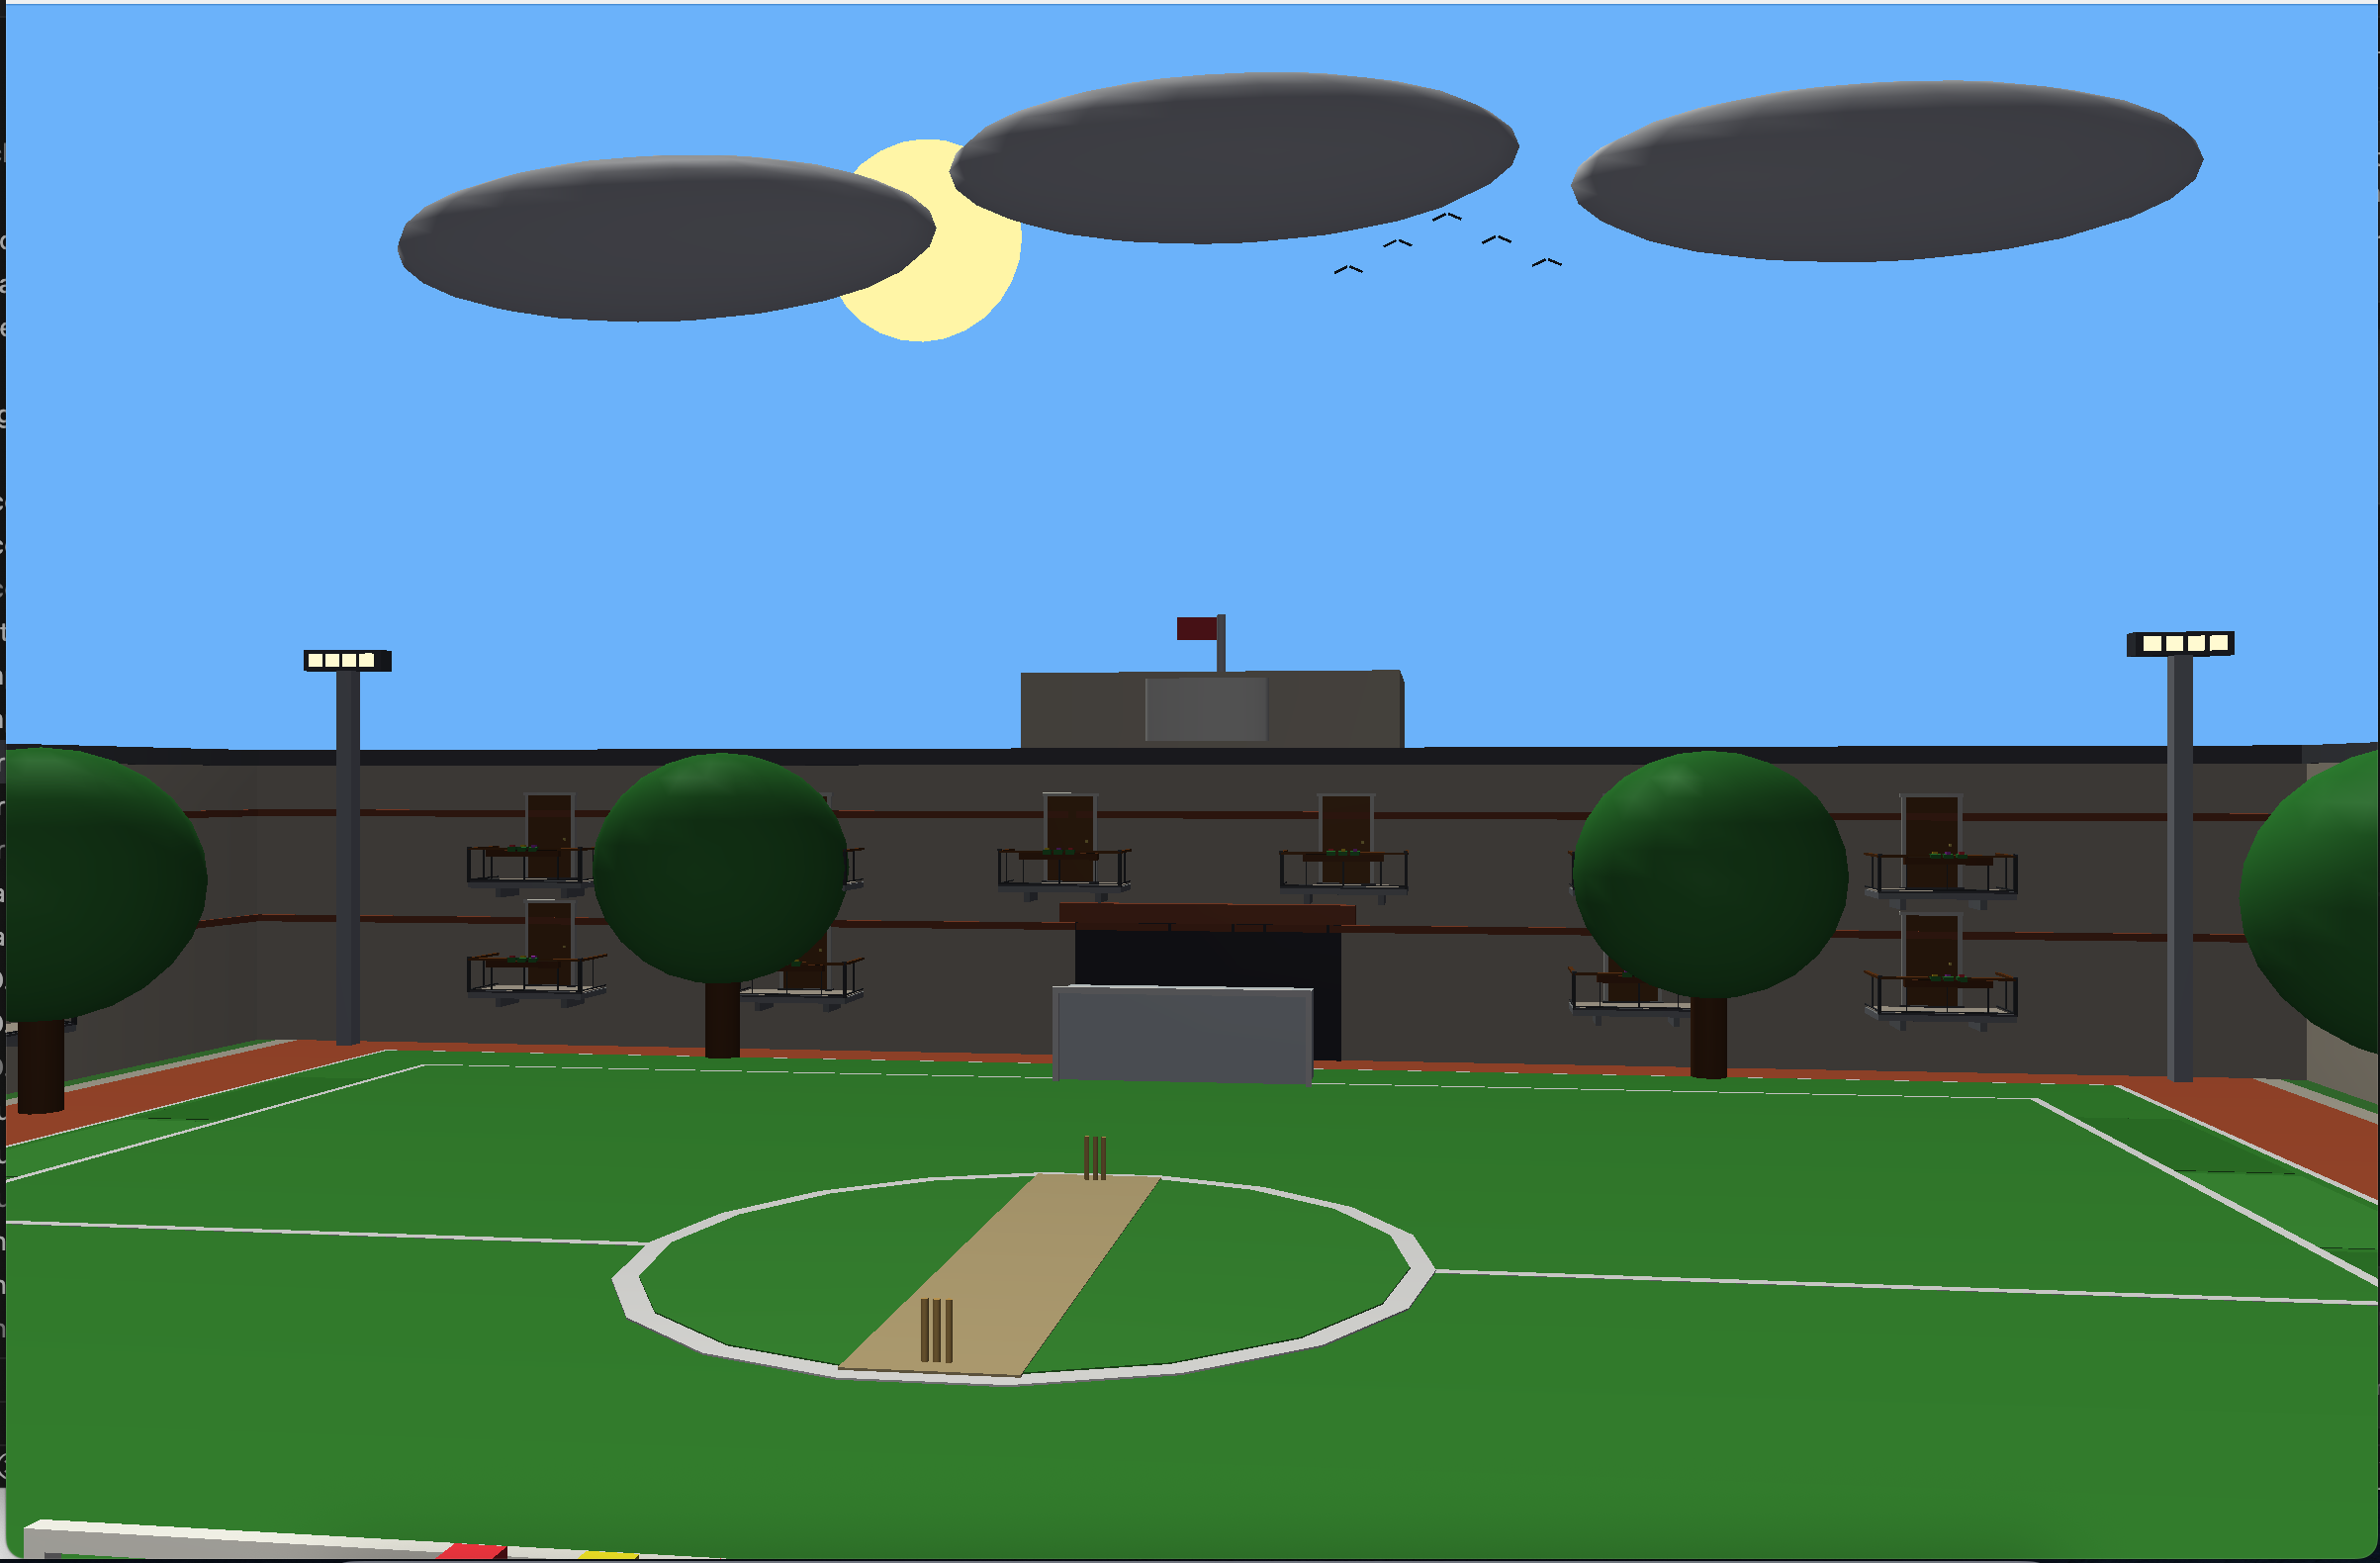
\includegraphics[width=\textwidth]{courtyard_panorama.png}
    \caption{Courtyard Panorama: Central cricket pitch with wickets, running track, trees, and sky.}
    \label{fig:courtyard_res}
\end{subfigure}
\vskip 8pt
\begin{subfigure}[b]{0.48\textwidth}
    \centering
    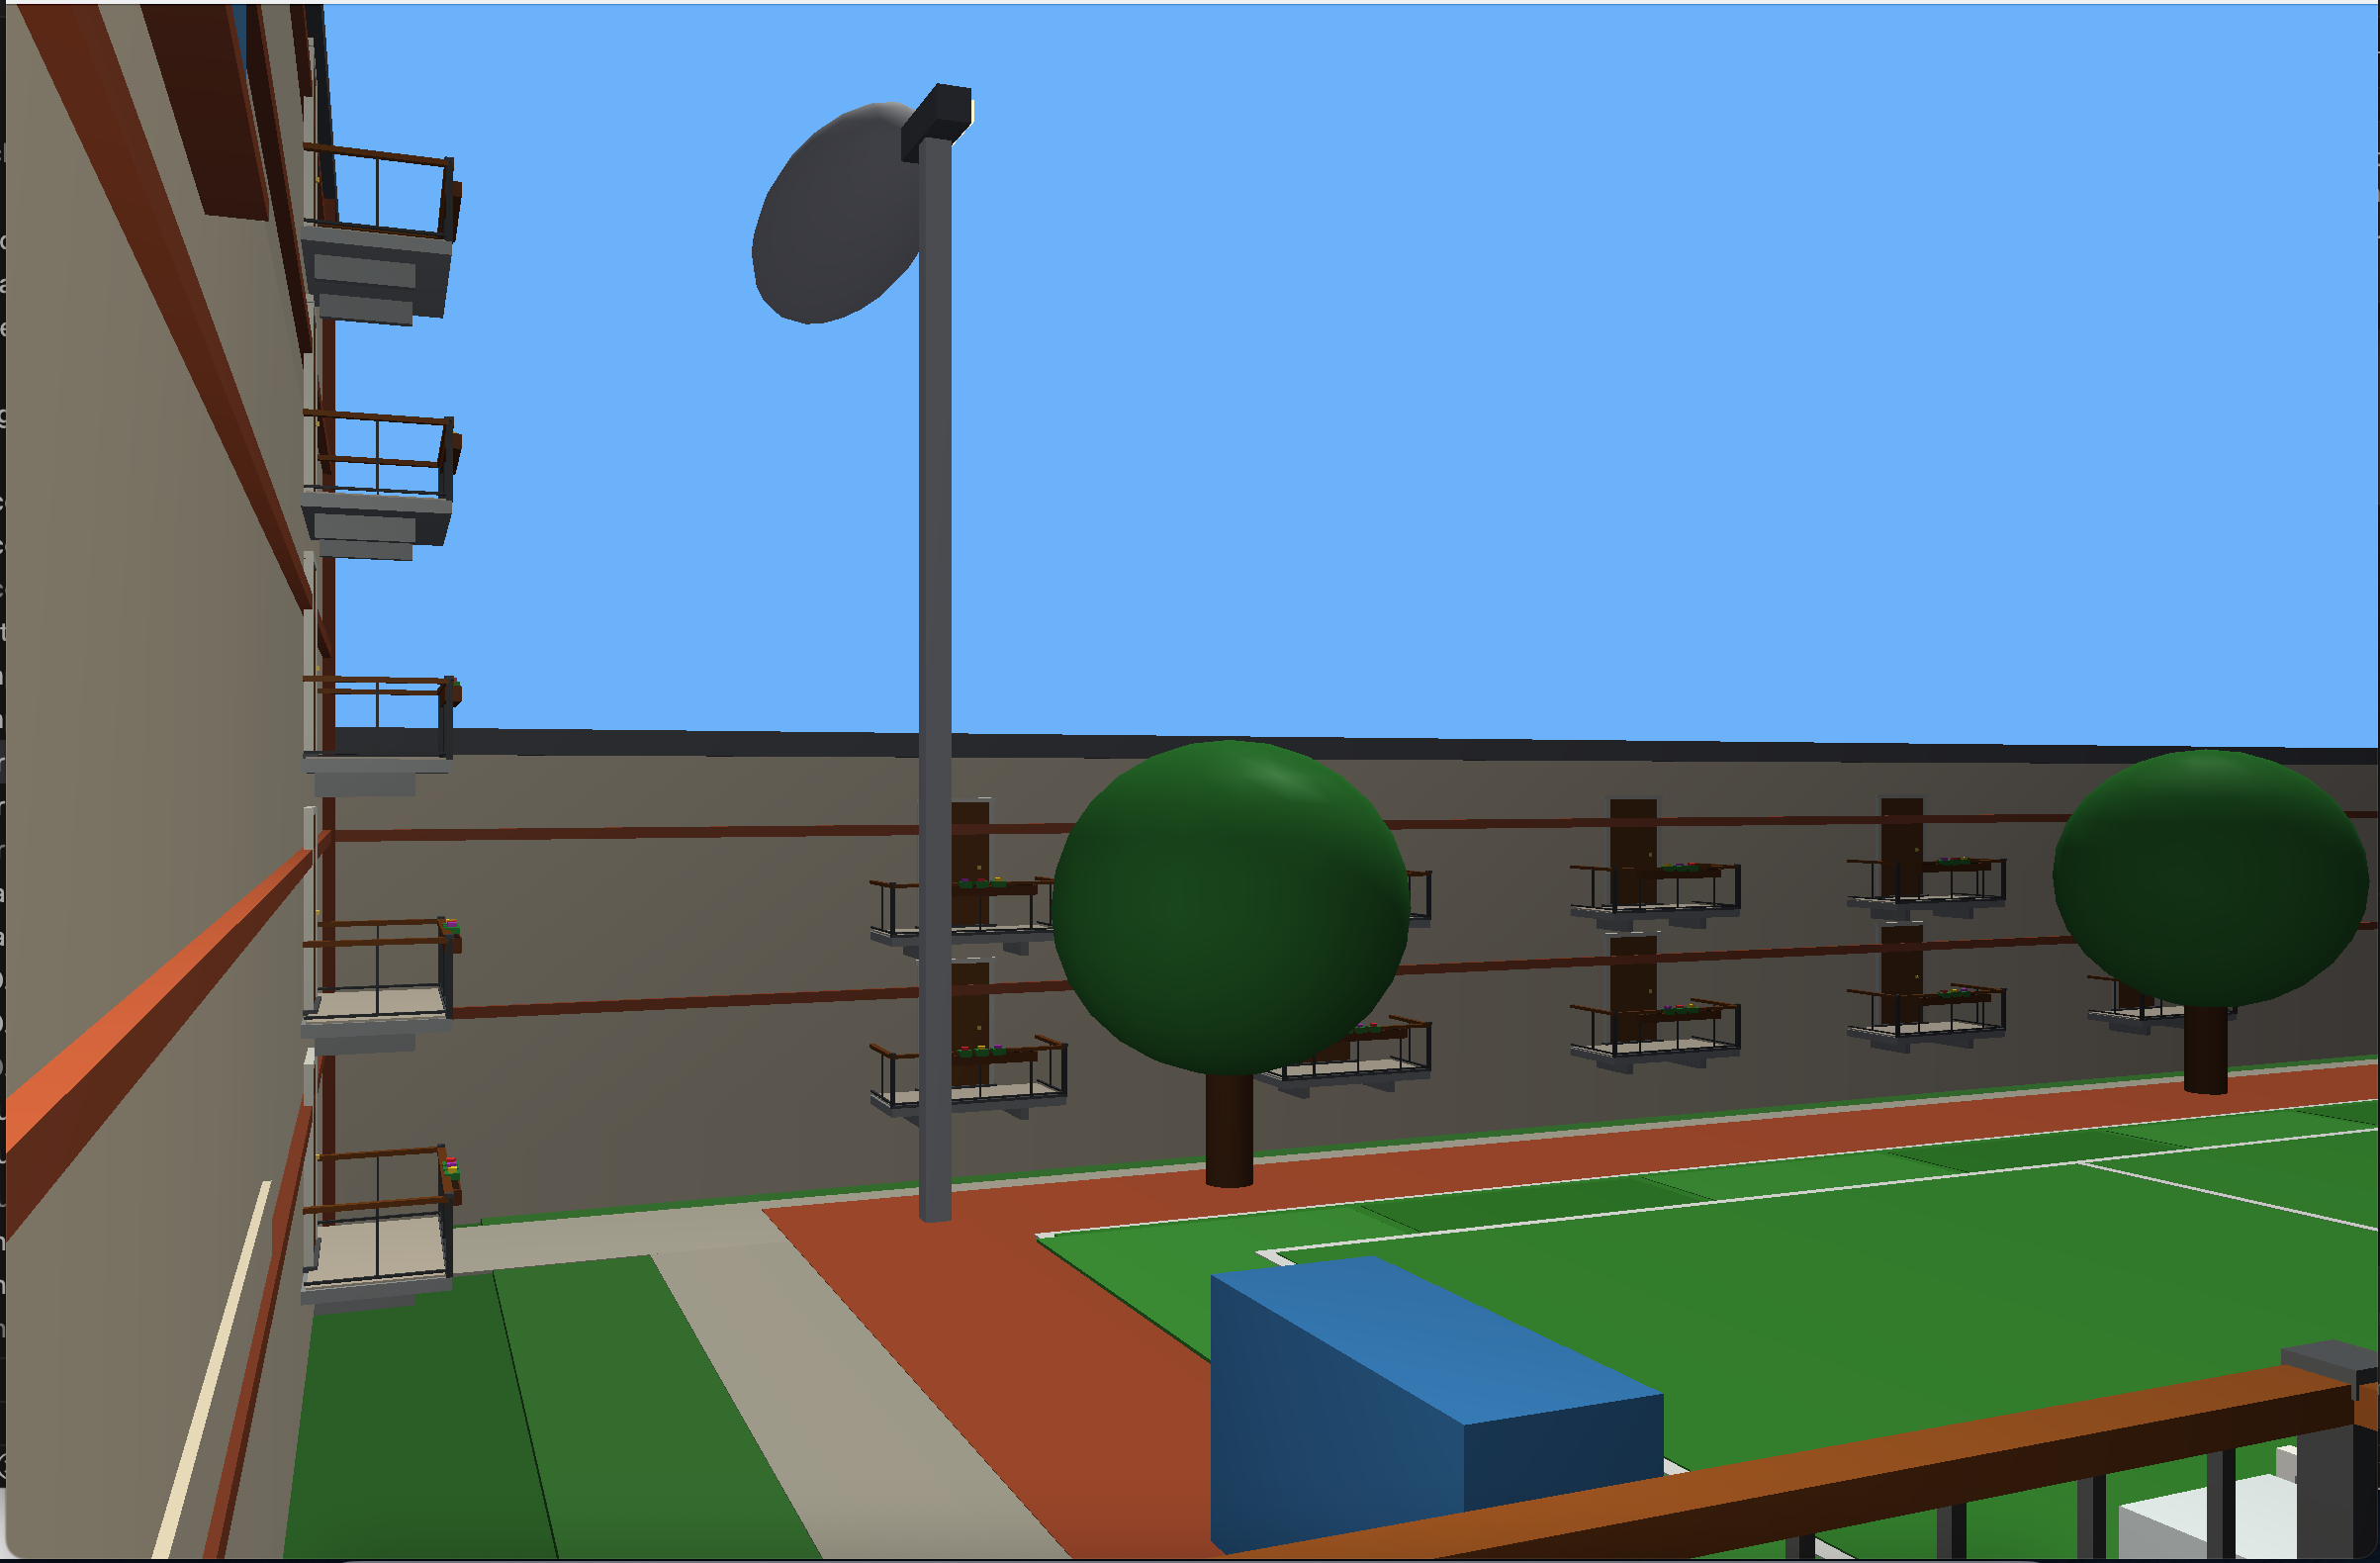
\includegraphics[width=\textwidth]{balcony_wing_view.png}
    \caption{South Wing Facade: Cantilever balconies overlooking the campus sports complex.}
    \label{fig:wing_res}
\end{subfigure}
\hfill
\begin{subfigure}[b]{0.48\textwidth}
    \centering
    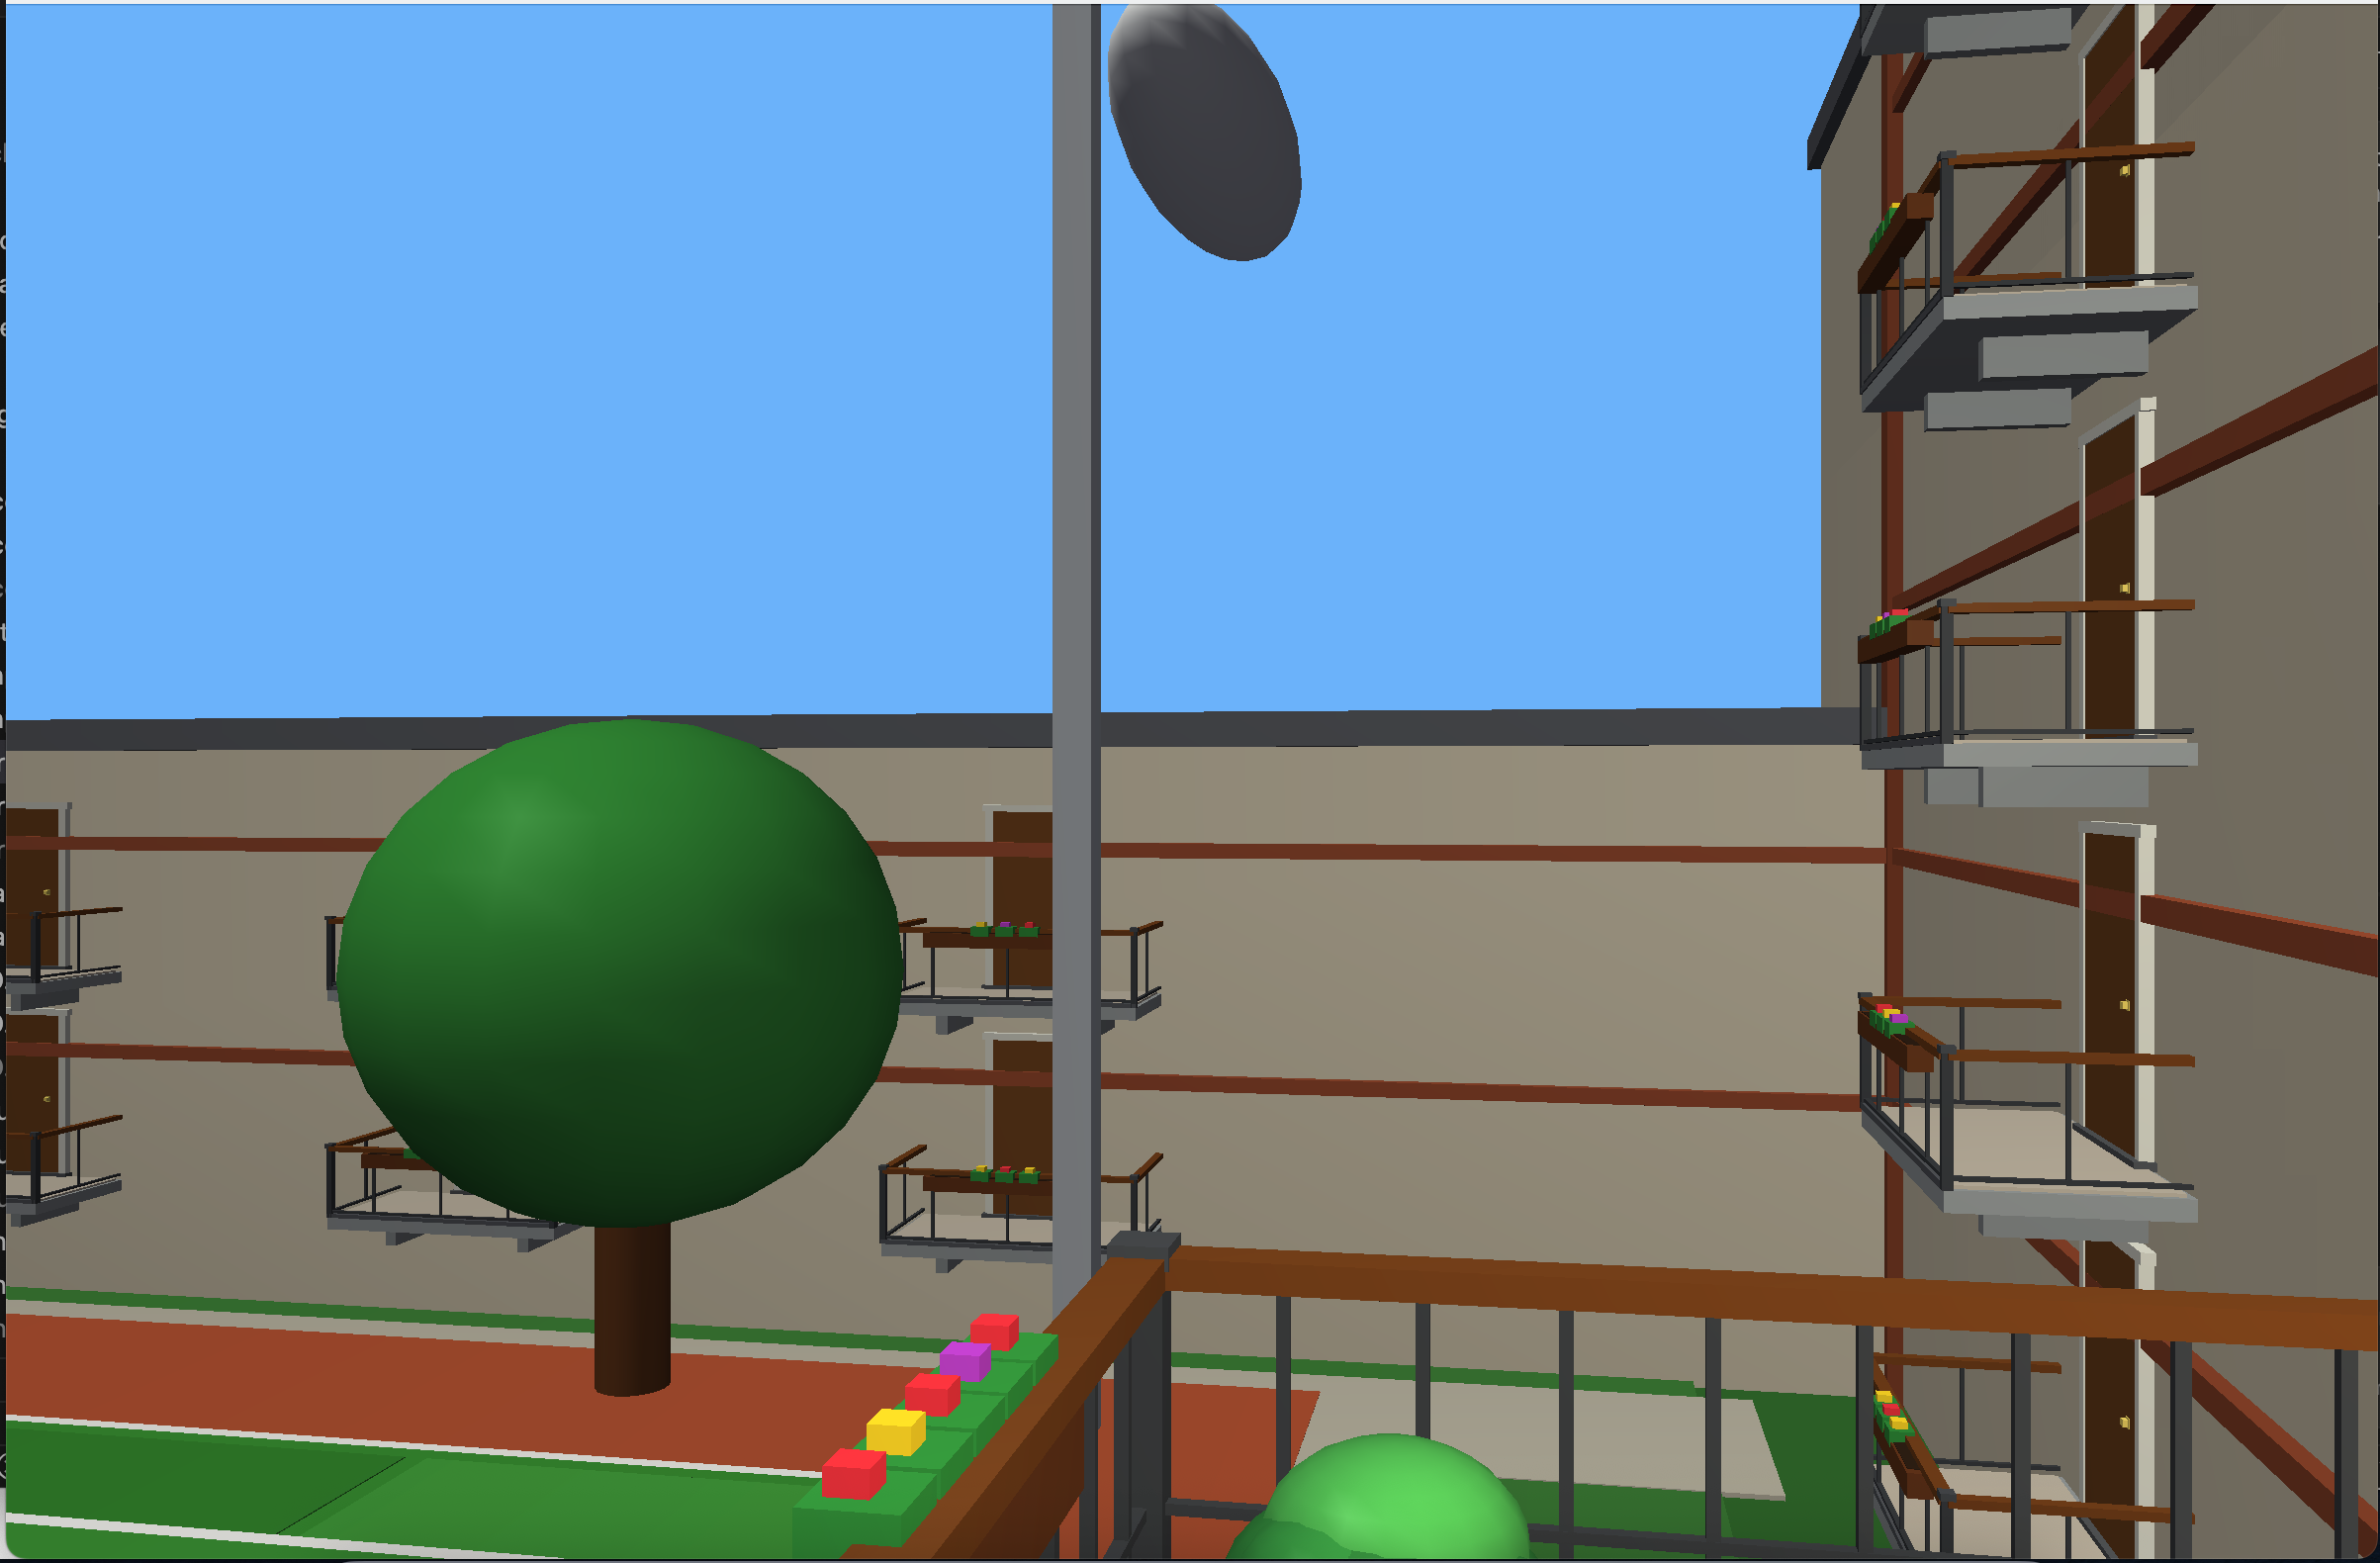
\includegraphics[width=\textwidth]{balcony_planters_view.png}
    \caption{Balcony Railing: Handrail planters with colorful blooms and floodlight mast vista.}
    \label{fig:planters_res}
\end{subfigure}
\caption{Architectural environmental showcase rendered in modern Core Profile OpenGL 3.3.}
\label{fig:arch_showcase}
\end{figure}

\vspace{0.1cm}
\begin{tcolorbox}[colback=boxbg, colframe=kuetblue, arc=3pt]
\textbf{Architectural Cohesion and Environmental Elements:}
The outdoor environment seamlessly expands upon the indoor dormitory experience. Looking down from the Room 304 balcony, users observe the red cinder running track surrounding the green soccer pitch, the accurately scaled cricket strip with stumps and bails, four 30m lattice floodlight masts, and the multi-story facade of Khan Jahan Ali Hall with cantilever balconies and vibrant floral planters.
\end{tcolorbox}

\clearpage

% ============================================================
% PAGE 15: CONCLUSION, DEFENSE & REFERENCES
% ============================================================
\section{Conclusion and Project Defense Guide}

\subsection{Summary of Technical Achievements}
This project successfully implemented an interactive 3D virtual walkthrough of Khan Jahan Ali Hall in modern Core Profile OpenGL 3.3 and C++. Key achievements include:
\begin{itemize}[leftmargin=1.2em, itemsep=1.0pt]
    \item \textbf{Mathematical Geometry Generation:} Complete scene constructed exclusively from three procedural primitive meshes (Cube, Sphere, Cylinder) requiring zero external model asset files.
    \item \textbf{Multi-Source Illumination Pipeline:} Combined directional sunlight with 6 distance-attenuated point lights, runtime-switchable Phong and Gouraud shading models, and emissive materials.
    \item \textbf{Interactive Kinematics:} Real-time exponential door swing animations, dual-motion oscillating table fan mechanics, and multi-zone portal navigation with collision prevention.
    \item \textbf{Z-Fighting Prevention:} Clean architectural layering ensuring artifact-free rendering across large corridor runner strips and complex quad athletic fields.
\end{itemize}

\subsection{Project Showcase and Defense Explanation Guide}
During evaluation, the application can be demonstrated using the following sequence:
\begin{enumerate}[leftmargin=1.2em, itemsep=1.0pt]
    \item \textbf{Primitive Mesh Construction:} Explain how the Unit Cube, UV Sphere, and Cylinder were coded in \texttt{Primitives.cpp} using parametric equations and vector cross products for normal computation. Highlight the EBO index optimization saving GPU memory.
    \item \textbf{Lighting and Shading Demonstration:} Press $G$ to switch to Gouraud Shading and point out polygonal highlight degradation on the table fan and bedposts; press $P$ to restore per-pixel Phong Shading.
    \item \textbf{Switchboard \& Attenuation Demo:} Toggle keys $1, 2, 3, 4$ to demonstrate independent point light deactivation and show corresponding LED color changes on the 4-gang switchboard. Turn off all lights to showcase dark room mode.
    \item \textbf{Kinematics and Portals:} Press $O$ to show smooth exponential door opening; walk through the doorway portal to showcase the outdoor quad sports ground, cricket pitch, and residential hall wings.
\end{enumerate}

\subsection{Future Architectural Extensions}
Future enhancements could incorporate texture mapping with normal bump maps, shadow mapping using depth framebuffer objects (FBOs), ambient occlusion, and audio emitters attached to the oscillating fan and doors.

\vspace{0.2cm}
\renewcommand{\refname}{\normalsize\color{kuetnavy}\textbf{References}}
\begin{thebibliography}{9}
\setlength{\itemsep}{0pt}
\setlength{\parskip}{0pt}
\scriptsize
\bibitem{learnopengl}
J. de Vries, \textit{LearnOpenGL: Learn Modern OpenGL Graphics Programming}, 2020. \url{https://learnopengl.com/}.
\bibitem{rtr4}
T. Akenine-M{\"o}ller, E. Haines, and N. Hoffman, \textit{Real-Time Rendering}, 4th ed., CRC Press, 2018.
\bibitem{opengl_spec}
Khronos Group, \textit{OpenGL 3.3 Core Profile Specification}, 2010.
\bibitem{glm_lib}
G-Truc Creation, \textit{OpenGL Mathematics (GLM) Library}, \url{https://github.com/g-truc/glm}.
\bibitem{kuet_cse}
Department of CSE, \textit{CSE 4102: Computer Graphics and Image Processing Laboratory Manual}, KUET, 2026.
\end{thebibliography}

\end{document}
